\documentclass[letterpaper,11pt]{article}

% --- PAQUETES DE IDIOMA
\usepackage[spanish,mexico]{babel}
\addto\captionsspanish{\renewcommand{\contentsname}{Indice}}
\usepackage[utf8]{inputenc}
\usepackage{pmboxdraw}
\usepackage{csquotes}
\usepackage{iftex}

\usepackage{pdfpages}

% --- PAQUETES MATEMÁTICOS --
\usepackage{amsmath}
\usepackage{cancel}
\usepackage{mathrsfs}

% --- PAQUETES GRÁFICOS Y DE DISEÑO ---
\usepackage{graphicx}
\usepackage{float}
\usepackage{placeins}
\usepackage{needspace}
\usepackage{subcaption}
\usepackage[table]{xcolor}
\usepackage{makecell}
\usepackage{array}
\usepackage{tikz}
\usetikzlibrary{shapes.geometric, shapes.multipart, positioning, arrows.meta, calc, shadows, decorations.pathreplacing,babel}

% --- LISTAS ---
\usepackage{enumitem}

% --- PAQUETES DE CÓDIGO ---
\usepackage{listings}
% Configuración del estilo de listings
\definecolor{codebg}{rgb}{0.95,0.95,0.95}   
\definecolor{keyword}{rgb}{0.0,0.2,0.6}     
\definecolor{comment}{rgb}{0.25,0.5,0.35}   
\definecolor{string}{rgb}{0.6,0.0,0.0}      
\definecolor{number}{rgb}{0.5,0.0,0.5}      
\definecolor{codegray}{rgb}{0.5,0.5,0.5}
\definecolor{codepurple}{rgb}{0.58,0,0.82}
\definecolor{backcolour}{rgb}{0.95,0.95,0.95}
\definecolor{cmdblue}{RGB}{0, 114, 188}
\definecolor{cmdred}{RGB}{204, 0, 0}       
\definecolor{cmdgreen}{RGB}{13, 165, 13}   
\definecolor{cmdgray}{RGB}{128, 128, 128} 
\definecolor{bgcode}{RGB}{248, 248, 248} 
\definecolor{bgTerminal}{RGB}{30, 30, 30}
\definecolor{textTerminal}{RGB}{230, 230, 230}




\lstset{
  backgroundcolor=\color{backcolour},
  basicstyle=\ttfamily\small,
  keywordstyle=\color{blue}\bfseries,
  stringstyle=\color{codepurple},
  commentstyle=\color{codegray}\itshape,
  numbers=left,
  numberstyle=\tiny\color{codegray},
  frame=single,
  rulecolor=\color{black},
  breaklines=true,
  tabsize=4,
  showstringspaces=false,
  literate={á}{{\'a}}1
           {é}{{\'e}}1
           {í}{{\'i}}1
           {ó}{{\'o}}1
           {ú}{{\'u}}1
           {Á}{{\'A}}1
           {É}{{\'E}}1
           {Í}{{\'I}}1
           {Ó}{{\'O}}1
           {Ú}{{\'U}}1
           {ñ}{{\~n}}1
           {Ñ}{{\~N}}1
           {¿}{{\textquestiondown}}1
           {¡}{{\textexclamdown}}1
}

% Estilo para código en C
\lstdefinestyle{cstyle}{
  language=C,
  backgroundcolor=\color{backcolour},
  basicstyle=\ttfamily\small,
  keywordstyle=\color{blue}\bfseries,
    keywordstyle=[2]\color{yellow!70!orange}\bfseries,
    morekeywords=[2]{MPI_Init,MPI_Comm_size,MPI_Comm_rank,MPI_Send,MPI_Recv,MPI_Scatter,MPI_Gather,MPI_Bcast,MPI_Reduce,MPI_Finalize},
    emph={printf},
    emphstyle=\color{blue}\bfseries,
  stringstyle=\color{codepurple},
  commentstyle=\color{codegray}\itshape,
  numbers=left,
  numberstyle=\tiny\color{codegray},
  frame=single,
  rulecolor=\color{black},
  breaklines=true,
  tabsize=4,
  showstringspaces=false
}

\lstdefinestyle{salidaLinpeas}{
    basicstyle=\ttfamily\scriptsize\color{textTerminal},
    backgroundcolor=\color{bgTerminal},
    breaklines=true,
    breakatwhitespace=true,
    frame=single,
    rulecolor=\color{black!50},
    numbers=none,
    showstringspaces=false,
    tabsize=4,
    xleftmargin=0.5cm,
    xrightmargin=0.5cm,
    extendedchars=false,
    literate={═}{{\textSFxliii}}1
             {║}{{\textSFxxiv}}1
             {╔}{{\textSFxxxix}}1
             {╗}{{\textSFxxv}}1
             {╚}{{\textSFxxxviii}}1
             {╝}{{\textSFxxvi}}1
             {╣}{{\textSFxxiii}}1
}  
\lstdefinestyle{consolaSeguridad}{
    language=bash,
    basicstyle=\ttfamily\footnotesize,
    backgroundcolor=\color{bgcode},
    % Herramientas y comandos de la práctica
    morekeywords={subfinder, make, scp, httpx, hydra, ssh, id, nuclei, dig, whois, grep, awk, sort, cut, sed, tr, nano, wc, head, echo, sudo, nmap, wget, curl, ip,
                  whoami, file, cat, cp, chown, chmod, sha256sum, apt-get, john, unshadow, su, pwnkit, uname, uniq, ps, route, ifconfig, find, tar, ping, nc, ls, bash, apt, remmina, systeminfo, findstr, dir, type, certutil, SHA256},
    alsoletter={-},
    keywordstyle=\color{cmdblue}\bfseries,
    % Palabras reservadas de ciclos Bash
    emph={for, in, do, done, while, read, if, then, fi},
    emphstyle=\color{cmdred}\bfseries,
    stringstyle=\color{cmdgreen},
    commentstyle=\color{cmdgray}\itshape,
    showstringspaces=false,
    breaklines=true,
    breakatwhitespace=false,
    frame=single,
    rulecolor=\color{black!30},
    numbers=none,
    literate={-}{{\textcolor{black}{-}}}1
             {ñ}{{\~n}}1
             {Ñ}{{\~N}}1
}


% Comandos utilizados dentro de la sesion remota de Windows
\lstdefinestyle{consolaWindows}{
    style=consolaSeguridad,
    language={},
    morekeywords={systeminfo,findstr,dir,type,certutil,SHA256},
    emph={},
    columns=fullflexible,
    keepspaces=true
}

% Definición del lenguaje Python para listings
\lstdefinelanguage[LAB]{Python}{
    morekeywords={False, None, True, and, as, assert, async, await, break,
                                class, continue, def, del, elif, else, except, finally,
                                for, from, global, if, import, in, is, lambda, nonlocal,
                                not, or, pass, raise, return, try, while, with, yield,
                                machine, Pin, PWM, ADC, Timer, sleep_ms, sleep_us},
    morecomment=[l]{\#},
    morestring=[b]",
    morestring=[b]',
    sensitive=true
}

% Definición del lenguaje Makefile para listings
\lstdefinelanguage{Makefile}{
    morekeywords={all, setup, clean, conversion-mod.so, pwnkit},
    morecomment=[l]{\#},
    morestring=[b]',
    morestring=[b]",
    sensitive=true
}

% Estilo para salidas de consola/terminal
\lstdefinestyle{output}{
  backgroundcolor=\color{black!5},
  basicstyle=\ttfamily\footnotesize,
  numbers=none,
  frame=single,
  rulecolor=\color{black!30},
  breaklines=true,
  tabsize=4,
  showstringspaces=false,
  xleftmargin=0.5cm,
  xrightmargin=0.5cm
}

% --- ESTILOS PARA DIAGRAMAS DE FLUJO (TIKZ) ---
\tikzset{
  startstop/.style={rectangle, rounded corners, minimum width=3cm, minimum height=1cm,text centered, draw=black, fill=red!30},
  process/.style={rectangle, minimum width=3cm, minimum height=1cm, text centered, draw=black, fill=orange!30},
  decision/.style={diamond, aspect=2, minimum width=3cm, minimum height=1cm, text centered, draw=black, fill=green!30},
  io/.style={trapezium, trapezium left angle=70, trapezium right angle=110, minimum width=3cm, minimum height=1cm, text centered, draw=black, fill=blue!30},
  arrow/.style={thick,->,>=stealth}
}


\definecolor{azulresultado}{HTML}{0072C6}
\definecolor{rojoacarreo}{HTML}{FF0000}

% --- RUTAS DE IMÁGENES ---
\graphicspath{{img/}{portada_img/}}

\definecolor{armblue}{RGB}{0, 113, 188}

% --- ÍNDICE CON PUNTOS ---
\usepackage{tocloft}
\renewcommand{\cftsecleader}{\cftdotfill{\cftdotsep}}

% --- CONFIGURACIÓN DE PÁGINA (GEOMETRÍA) ---
\usepackage[
    left=25mm, 
    right=25mm,
    top=35mm,
    bottom=30mm,
    headheight=77pt, 
    papersize={21.59cm,27.94cm}
]{geometry}

% --- FORMATO DE TEXTO ---
\usepackage{setspace}
\onehalfspacing
\usepackage{parskip} 
\usepackage{lipsum}  

% --- VARIABLES GLOBALES ---
\newcommand{\materia}{}

% --- ENCABEZADOS Y PIES DE PÁGINA ---
\usepackage{fancyhdr}
\pagestyle{fancy}
\fancyhf{} 
\fancyhead[L]{
\includegraphics[height=1.5cm]{portada_img/der.png}}
\fancyhead[R]{
\includegraphics[height=1.5cm]{portada_img/izq.png}}
\fancyfoot[C]{\thepage} 

\renewcommand{\headrulewidth}{0.4pt} 
\renewcommand{\footrulewidth}{0pt}  

% --- BIBLIOGRAFÍA ---
\usepackage[backend=biber, style=apa, sortcites, url=true]{biblatex}
\addbibresource{referencias.bib}

% --- HIPERVÍNCULOS ---
\usepackage{hyperref}
\hypersetup{
    colorlinks=true,
    linkcolor=blue,
    citecolor=blue,
    filecolor=magenta,
    urlcolor=cyan
}


\fancypagestyle{estiloindice}{
  \fancyhf{} 
  \fancyhead[L]{
\includegraphics[height=1.5cm]{portada_img/der.png}}
  \fancyhead[R]{
\includegraphics[height=1.5cm]{portada_img/izq.png}}
  \renewcommand{\headrulewidth}{0.4pt} 
  \renewcommand{\footrulewidth}{0pt}
}


% --- CADENAS DE HASHES: CONSERVAR CARACTERES Y PERMITIR SALTOS ---
\lstdefinestyle{hashCredencial}{
  style=output,
  basicstyle=\ttfamily\footnotesize,
  columns=fullflexible,
  keepspaces=true,
  breaklines=true,
  breakatwhitespace=false,
  xleftmargin=0pt,
  xrightmargin=0pt,
  postbreak=\mbox{\textcolor{codegray}{$\hookrightarrow$}\space}
}

\begin{document}
\setlength{\emergencystretch}{1em}
\hypersetup{pageanchor=false}
\thispagestyle{empty} % Sin encabezado ni pie en la portada

% --- ENCABEZADO DE PORTADA (TABLA DE 3 COLUMNAS) ---
\begin{center}
    % La tabla usa 'm' para centrar verticalmente las imagenes y el texto
    \begin{tabular}{m{0.15\textwidth} m{0.60\textwidth} m{0.15\textwidth}}
        % Logo Izquierdo (UNAM)
        
\includegraphics[width=2cm]{portada_img/der.png} & 
        
        % Titulo Central
        \centering\Huge\textbf{Universidad Nacional Autonoma de Mexico} &
        
        % Logo Derecho (Facultad)
        \raggedleft
\includegraphics[width=2cm]{portada_img/izq.png}
    \end{tabular}
\end{center}

\vspace{0.3cm}

% --- INFORMACION DEL REPORTE ---
\begin{center}
    {\LARGE \textbf{Facultad de Ingenieria}}\\[1cm]

    {\LARGE \textbf{Alumno:}}\\[0.3cm]
    {\Large Lara Hernandez Angel Husiel - 320060829} \\[1cm]


    {\LARGE \textbf{Seguridad informatica basica}} \\[1cm]

	{\LARGE Semestre: 2027-1} \\[1cm]
    
    {\LARGE \textbf{Practica 7}}\\[0.5cm]

    {\LARGE {Lateral Movement}}\\[1cm]


    {\Large \textbf{Fecha de Entrega:}}\\[0.2cm]
    {\Large 31 de Octubre del 2026 }
\end{center}
\newpage
{\hypersetup{linkcolor=black}\tableofcontents}
\thispagestyle{estiloindice}
\newpage
\thispagestyle{fancy}
\setcounter{page}{1}
\hypersetup{pageanchor=true}
\singlespacing
\section{Desarrollo}

\Needspace{8\baselineskip}
\subsection{Revision de la direccion IP y conectividad con webserver}

Primero revisamos la
direccion IP de nuestra maquina EvilBox. Para esto, el comando
que ponemos es el siguiente:

\begin{lstlisting}[style=consolaSeguridad]
ip a
\end{lstlisting}

Donde en este caso, la interfaz ens33 tiene la direccion
\texttt{192.168.177.128/24}, por lo que el segmento que vamos a
revisar es \texttt{192.168.177.0/24}. Despues de esto, utilizamos
nmap con el siguiente comando:

\begin{lstlisting}[style=consolaSeguridad]
sudo nmap -sP 192.168.177.0/24
\end{lstlisting}

\begin{figure}[H]
    \centering
    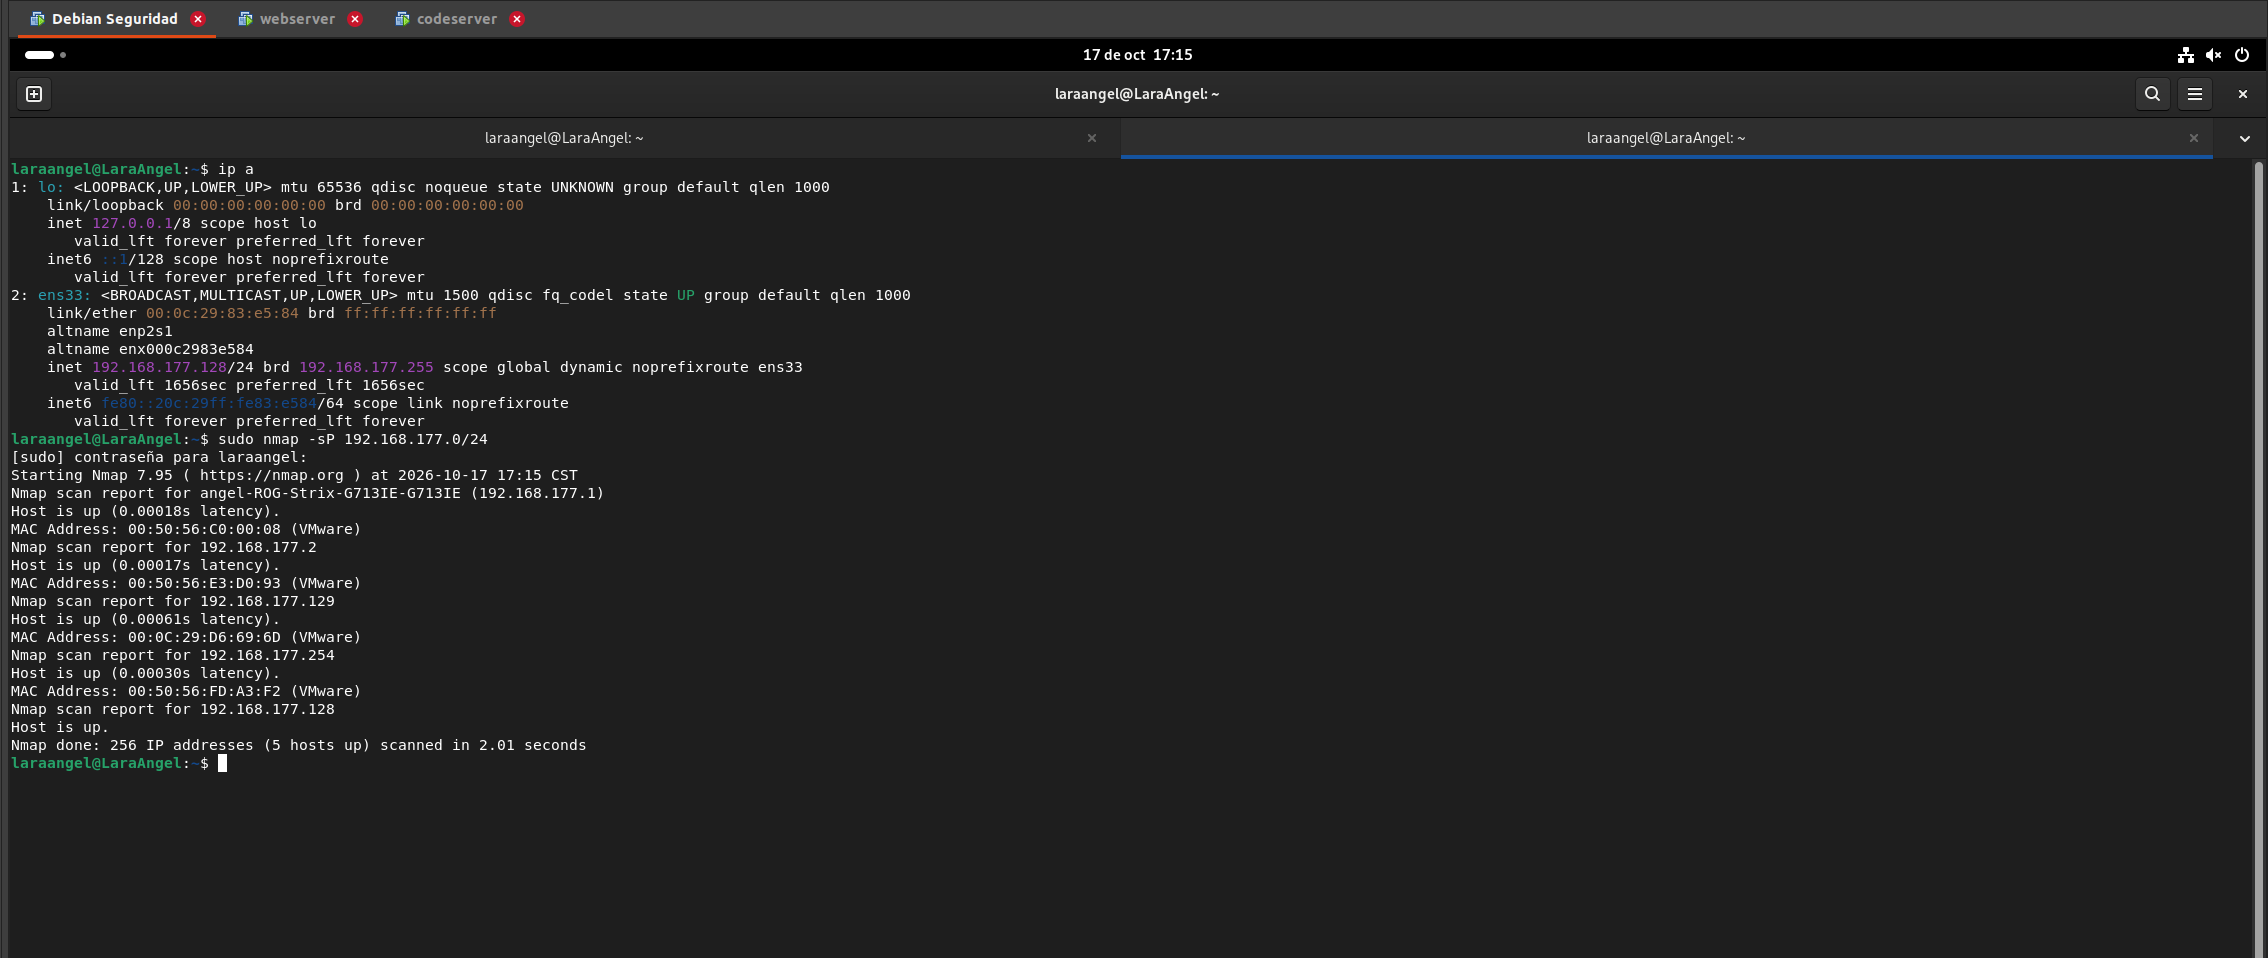
\includegraphics[width=\textwidth,trim=0bp 160bp 900bp 80bp,clip]{img/image1.png}
    \caption{Direccion IP de EvilBox y descubrimiento de los equipos activos.}
\end{figure}

Lo que hace este comando es identificar los equipos activos del
segmento de red. Donde \texttt{sudo} permite ejecutarlo con
permisos de administracion, \texttt{-sP} realiza el
descubrimiento de equipos y \texttt{/24} corresponde a la mascara
\texttt{255.255.255.0}. Esta opcion de nmap tambien se conoce
como \texttt{-sn}.

La salida nos arroja cinco equipos activos, incluyendo
\texttt{192.168.177.129}, que es la direccion de webserver
utilizada en las practicas anteriores. Por lo que, con esta
direccion continuamos con la conexion por SSH.

\Needspace{8\baselineskip}
\subsection{Conexion por SSH y prueba de comunicacion con codeserver}

Para poder conectarnos a webserver, utilizamos las credenciales
que se obtuvieron en la practica 3. Recordando que el usuario es
webadmin, la contraseña es toronto y el puerto SSH es el 13337,
el comando es el siguiente:

\begin{lstlisting}[style=consolaSeguridad]
ssh -p 13337 webadmin@192.168.177.129
\end{lstlisting}

Donde \texttt{-p} indica el puerto del servicio SSH y
\texttt{webadmin@192.168.177.129} indica el usuario y el equipo
al que nos conectamos. Despues en la consola se pone la
contraseña, siendo \texttt{toronto}.

\begin{figure}[H]
    \centering
    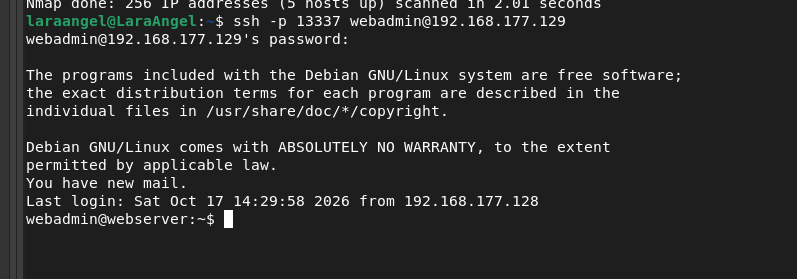
\includegraphics[width=\textwidth,trim=0bp 40bp 0bp 15bp,clip]{img/image2.png}
    \caption{Conexion por SSH desde EvilBox al equipo webserver.}
\end{figure}

Ahora bien, en la practica 6 se encontro otro equipo en la red
interna, siendo su direccion \texttt{10.0.0.201}. Para revisar si
webserver tiene comunicacion con este equipo, ponemos el
siguiente comando dentro de la sesion SSH:

\begin{lstlisting}[style=consolaSeguridad]
ping -c 6 10.0.0.201
\end{lstlisting}

Lo que hace ping es enviar solicitudes ICMP para comprobar si se
reciben respuestas. Donde la bandera \texttt{-c 6} limita la
prueba a seis paquetes y al final se pone la direccion de
codeserver.

\begin{lstlisting}[style=output]
6 packets transmitted, 6 received, 0% packet loss
\end{lstlisting}

\begin{figure}[H]
    \centering
    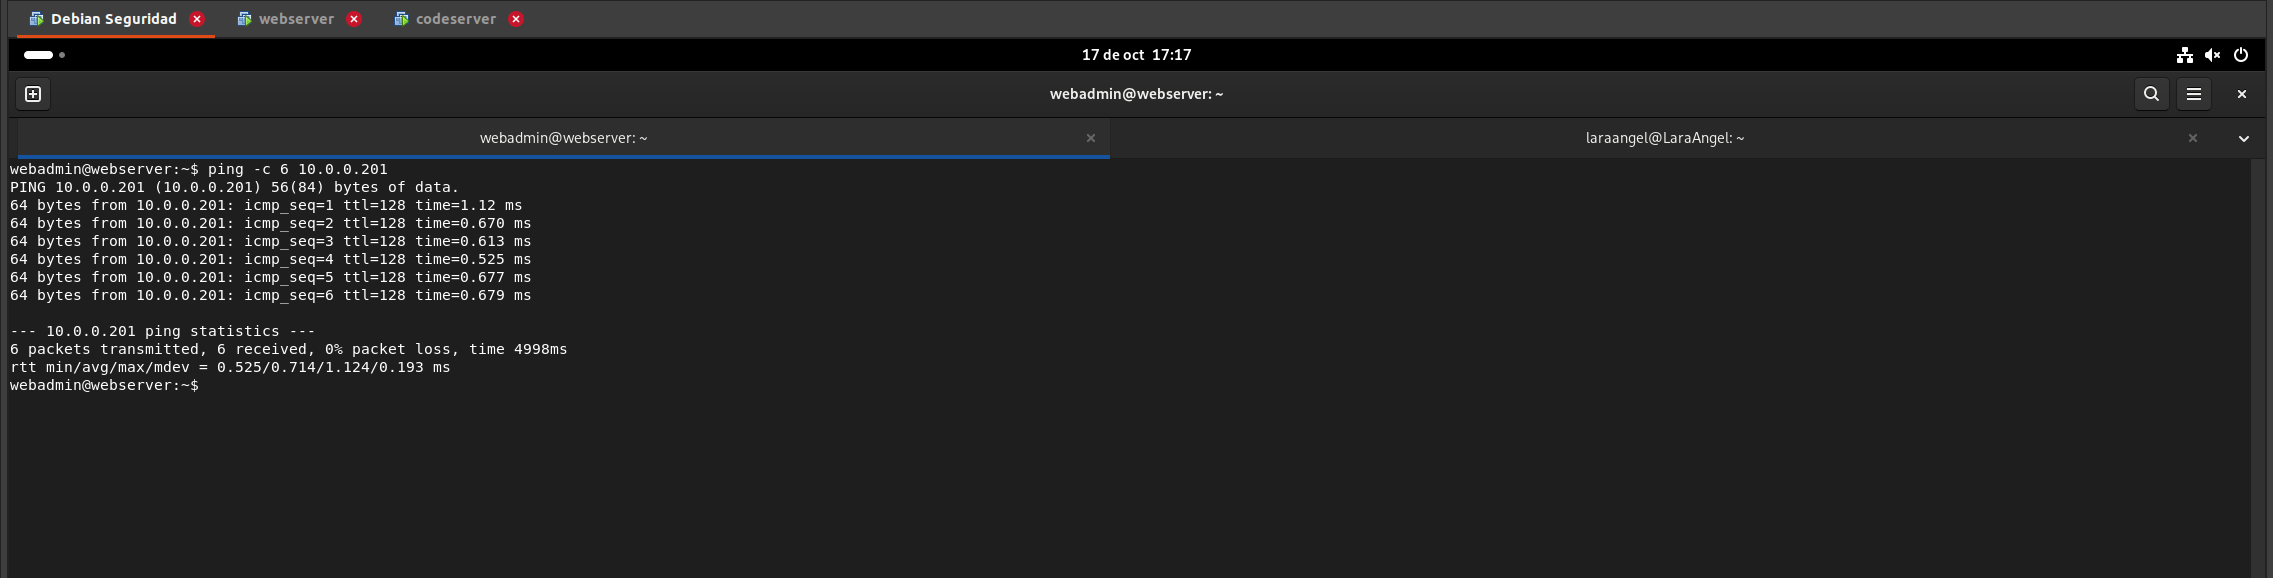
\includegraphics[width=\textwidth,trim=0bp 165bp 1100bp 145bp,clip]{img/image3.png}
    \caption{Prueba de conectividad desde webserver hacia codeserver.}
\end{figure}

Donde en este caso, se enviaron seis paquetes y se recibieron los
seis, con una perdida del 0\%. Con esto podemos ver que webserver
si tiene comunicacion con codeserver por la red interna.

Despues de esto, hacemos la misma prueba desde otra terminal de
EvilBox, utilizando el mismo comando:

\begin{lstlisting}[style=consolaSeguridad]
ping -c 6 10.0.0.201
\end{lstlisting}

\begin{lstlisting}[style=output]
6 packets transmitted, 0 received, 100% packet loss
\end{lstlisting}

\begin{figure}[H]
    \centering
    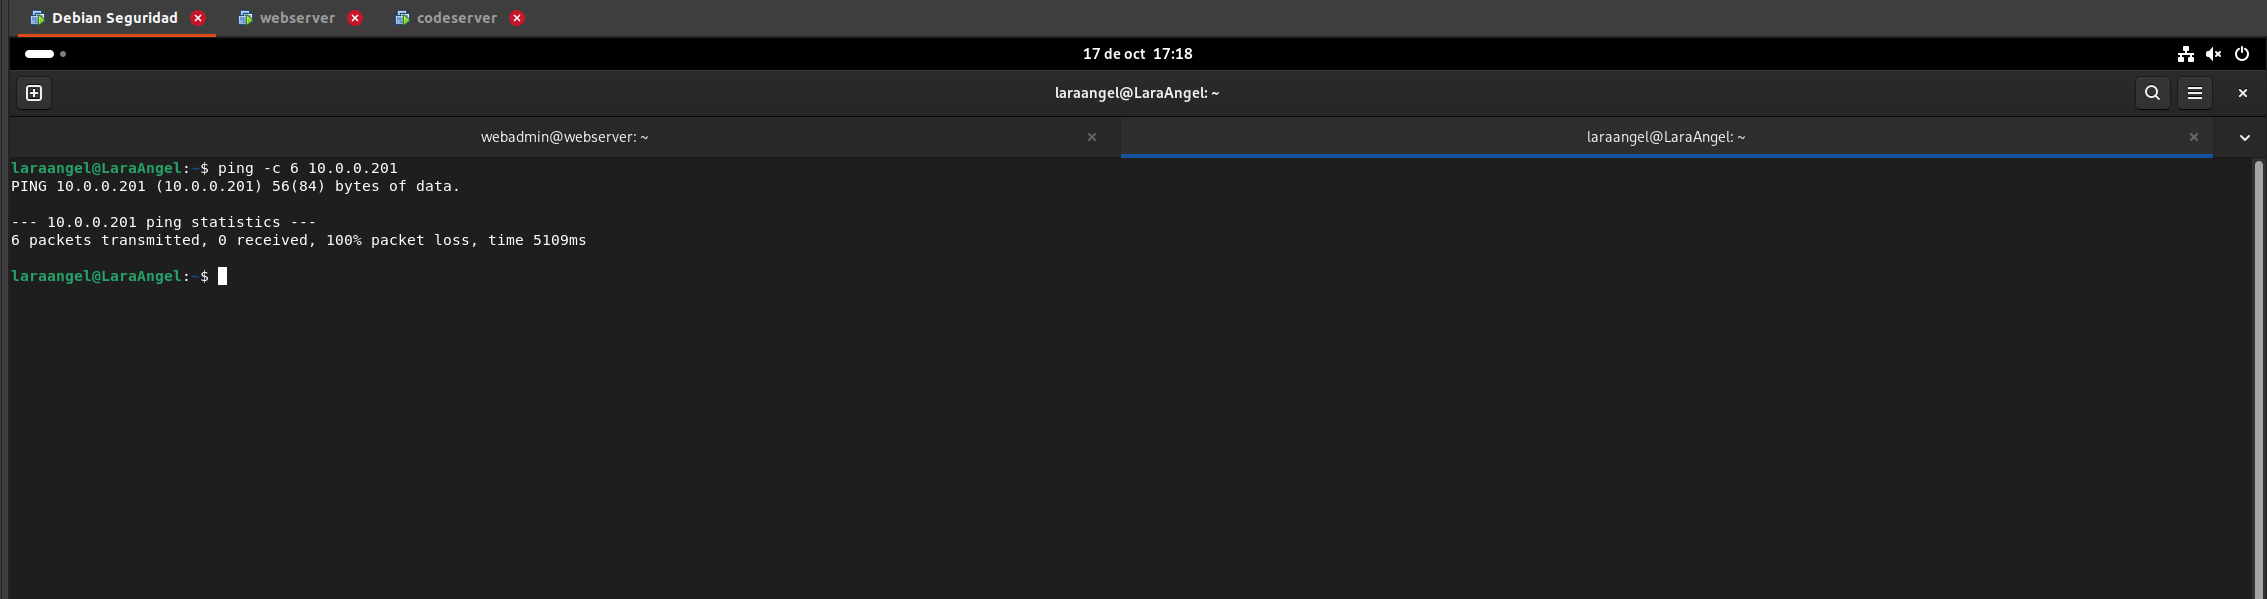
\includegraphics[width=\textwidth,trim=0bp 290bp 1100bp 145bp,clip]{img/image4.png}
    \caption{Prueba de conectividad desde EvilBox hacia codeserver.}
\end{figure}

No obstante, desde EvilBox no se recibio ninguna respuesta y la
perdida fue del 100\%. Esto coincide con la configuracion que
revisamos en la practica anterior: EvilBox y webserver comparten
la red \texttt{192.168.177.0/24}, mientras que codeserver se
encuentra en la red interna \texttt{10.0.0.0/24}.

Ademas de que, webserver tiene una segunda interfaz, eth1, con la
direccion \texttt{10.0.0.78}, por lo que puede comunicarse con
ambos segmentos. Para continuar, vamos a utilizar esa conexion de
webserver como paso intermedio hacia codeserver.

\Needspace{8\baselineskip}
\subsection{Creacion del tunel SSH con un puerto local}

Para poder conectarnos al escritorio remoto de codeserver desde
EvilBox, utilizamos un tunel SSH. Para esto, el comando completo
es el siguiente:

\begin{lstlisting}[style=consolaSeguridad]
ssh -p 13337 -L 3389:10.0.0.201:3389 webadmin@192.168.177.129
\end{lstlisting}

Donde la primera parte, \texttt{ssh -p 13337}, establece la
conexion SSH con webserver. Despues, la bandera \texttt{-L}
configura el reenvio de un puerto local hacia una direccion y un
puerto que se pueden alcanzar desde el servidor SSH.

La parte \texttt{3389:10.0.0.201:3389} esta formada por tres
valores, los cuales corresponden a lo siguiente:

\begin{itemize}
    \item \textbf{Primer 3389:} puerto local que se habilita en EvilBox.
    \item \textbf{10.0.0.201:} direccion de codeserver en la red interna.
    \item \textbf{Segundo 3389:} puerto del servicio RDP de codeserver.
\end{itemize}

Por ultimo, \texttt{webadmin@192.168.177.129} indica la cuenta
que se utiliza para abrir el tunel en webserver. Para esta
conexion se escribe la contraseña de webadmin, siendo toronto, y
se mantiene abierta la sesion SSH mientras se utiliza el
escritorio remoto.

\begin{figure}[H]
    \centering
    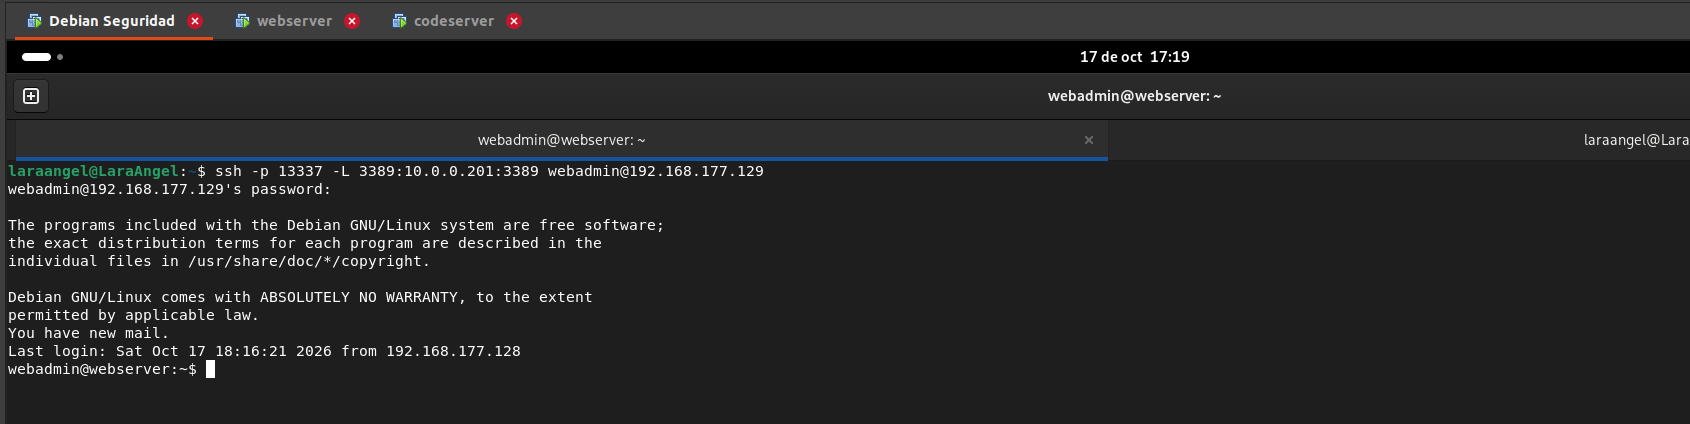
\includegraphics[width=\textwidth]{img/image5.png}
    \caption{Creacion del tunel SSH hacia el puerto RDP de codeserver.}
\end{figure}

Con esto, cuando una aplicacion de EvilBox se conecta a
\texttt{127.0.0.1:3389}, el trafico se envia por la conexion SSH
hasta webserver y desde ese equipo se abre la conexion hacia
\texttt{10.0.0.201:3389}. Por lo que no es necesario que EvilBox
tenga acceso directo a toda la red interna.

Ahora bien, el tunel que se creo reenvia conexiones TCP de ese
puerto. Esto no agrega una ruta general hacia la red interna ni
hace que ping empiece a responder, ya que ping utiliza ICMP.

\Needspace{8\baselineskip}
\subsection{Comprobacion del puerto local con netcat}

Para revisar que el puerto local quedo disponible, abrimos otra
terminal de EvilBox y utilizamos el siguiente comando:

\begin{lstlisting}[style=consolaSeguridad]
nc -zv 127.0.0.1 3389
\end{lstlisting}

Donde \texttt{nc} es la herramienta netcat, \texttt{-z} comprueba
el puerto sin intercambiar datos de aplicacion y \texttt{-v}
muestra el resultado de la conexion. La direccion
\texttt{127.0.0.1} corresponde al propio EvilBox y el puerto 3389
es el que se habilito con la bandera -L.

\begin{lstlisting}[style=output]
localhost [127.0.0.1] 3389 (ms-wbt-server) open
\end{lstlisting}

\begin{figure}[H]
    \centering
    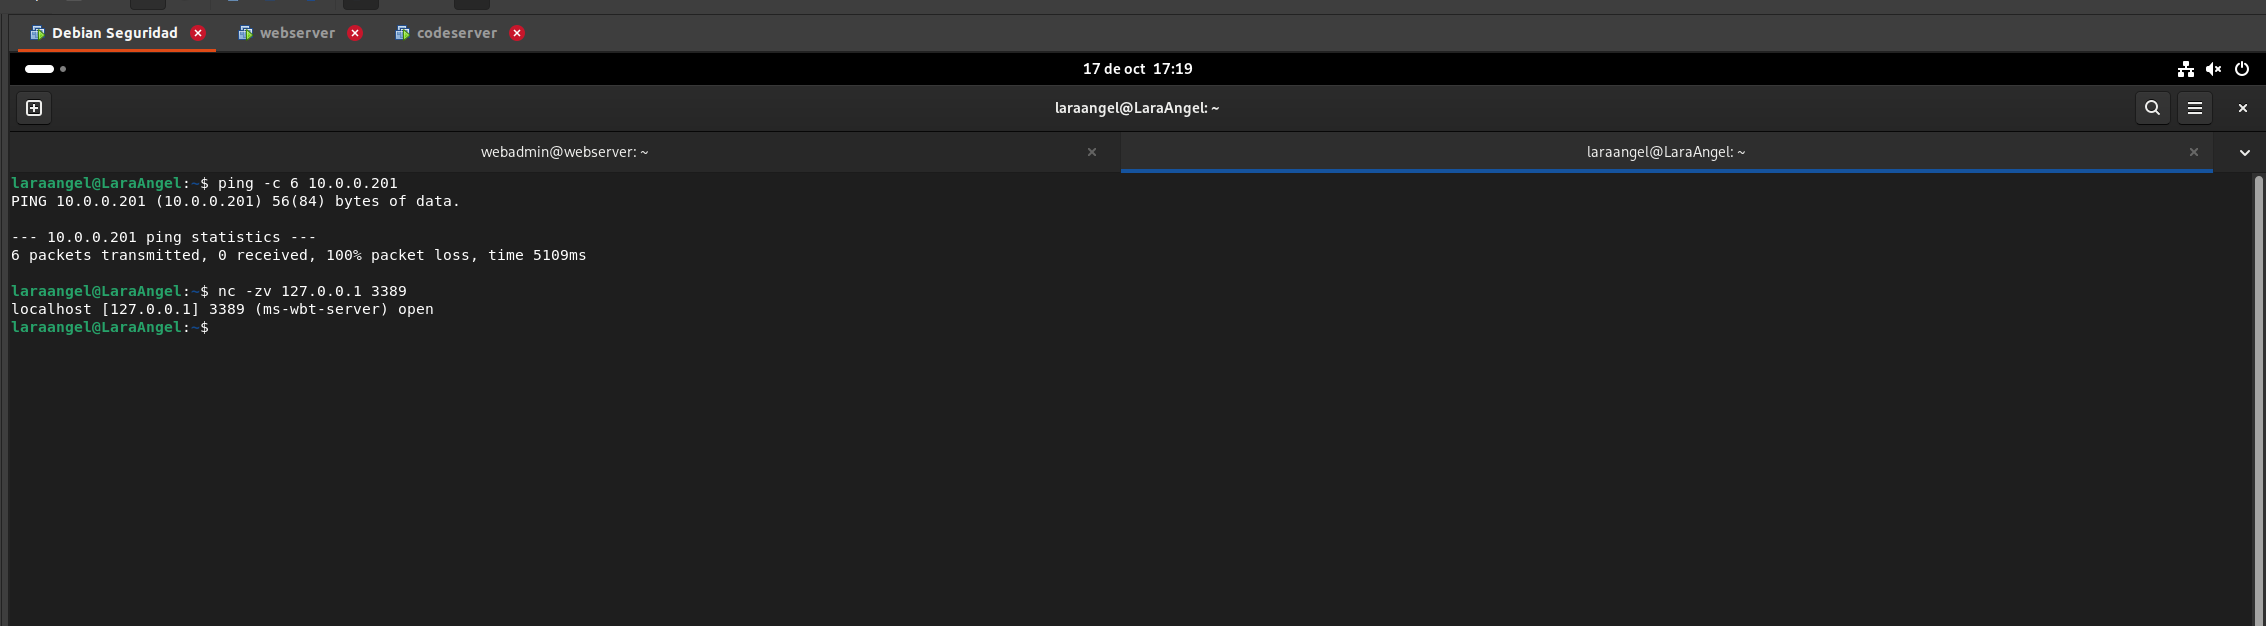
\includegraphics[width=\textwidth,trim=0bp 306bp 1650bp 280bp,clip]{img/image6.png}
    \caption{Comprobacion del puerto 3389 local mediante netcat.}
\end{figure}

Donde en este caso, el resultado open indica que se pudo abrir la
conexion TCP al puerto local. Con esto ya se puede utilizar ese
puerto desde Remmina; la comprobacion completa del acceso al otro
equipo se realiza al iniciar la sesion RDP.

\Needspace{8\baselineskip}
\subsection{Instalacion y ejecucion de Remmina}

Para establecer la conexion grafica con codeserver, utilizamos
Remmina. Para esto, primero se instalaron la herramienta y el
complemento para RDP en EvilBox con el siguiente comando:

\begin{lstlisting}[style=consolaSeguridad]
sudo apt update && sudo apt install remmina remmina-plugin-rdp -y
\end{lstlisting}

Lo que hace \texttt{apt update} es actualizar la informacion de
los paquetes disponibles. Despues, \texttt{apt install} instala
Remmina junto con \texttt{remmina-plugin-rdp}, que es el
complemento necesario para utilizar ese protocolo. Los simbolos
\texttt{\&\&} hacen que la instalacion se ejecute si la
actualizacion termino correctamente, y \texttt{-y} acepta la
confirmacion de los paquetes.

\begin{figure}[H]
    \centering
    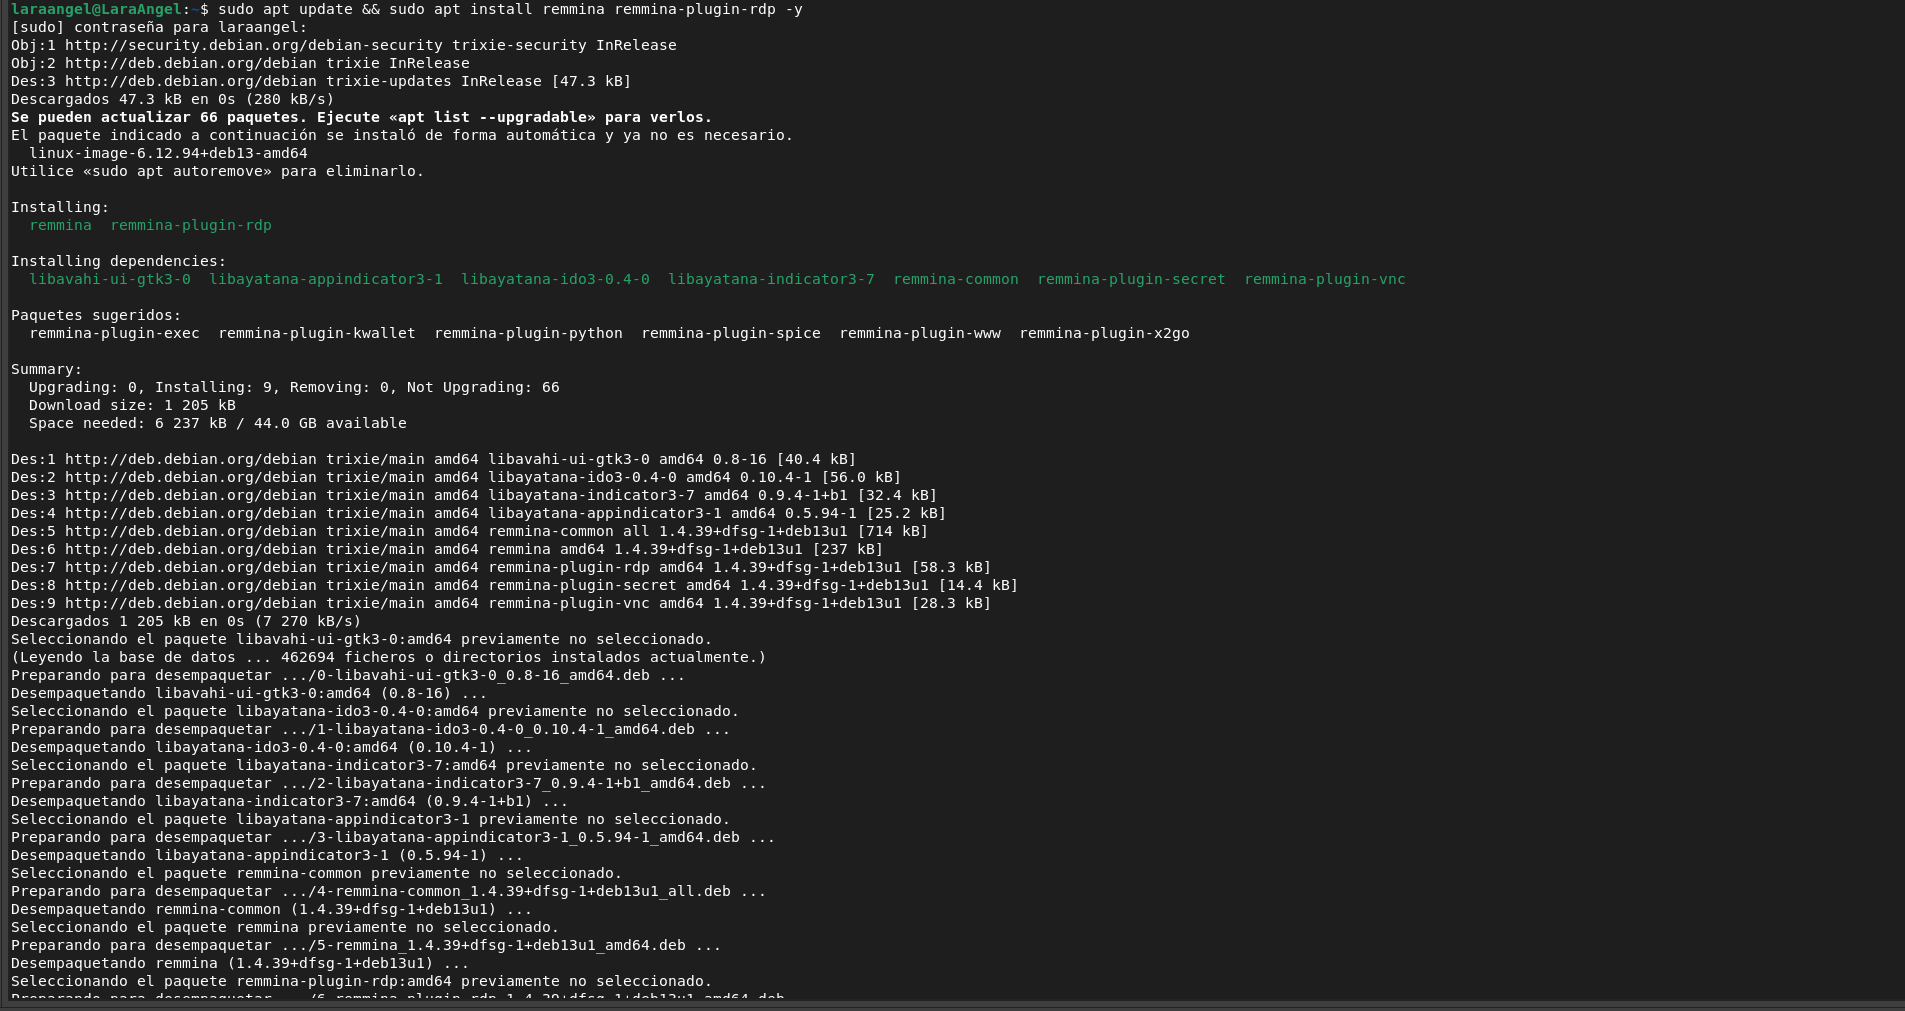
\includegraphics[width=0.95\textwidth]{img/image7.png}
    \caption{Instalacion de Remmina y del complemento de escritorio remoto.}
\end{figure}

Despues de esto, para abrir el programa se utiliza el siguiente
comando desde la terminal de EvilBox:

\begin{lstlisting}[style=consolaSeguridad]
remmina
\end{lstlisting}

\begin{figure}[H]
    \centering
    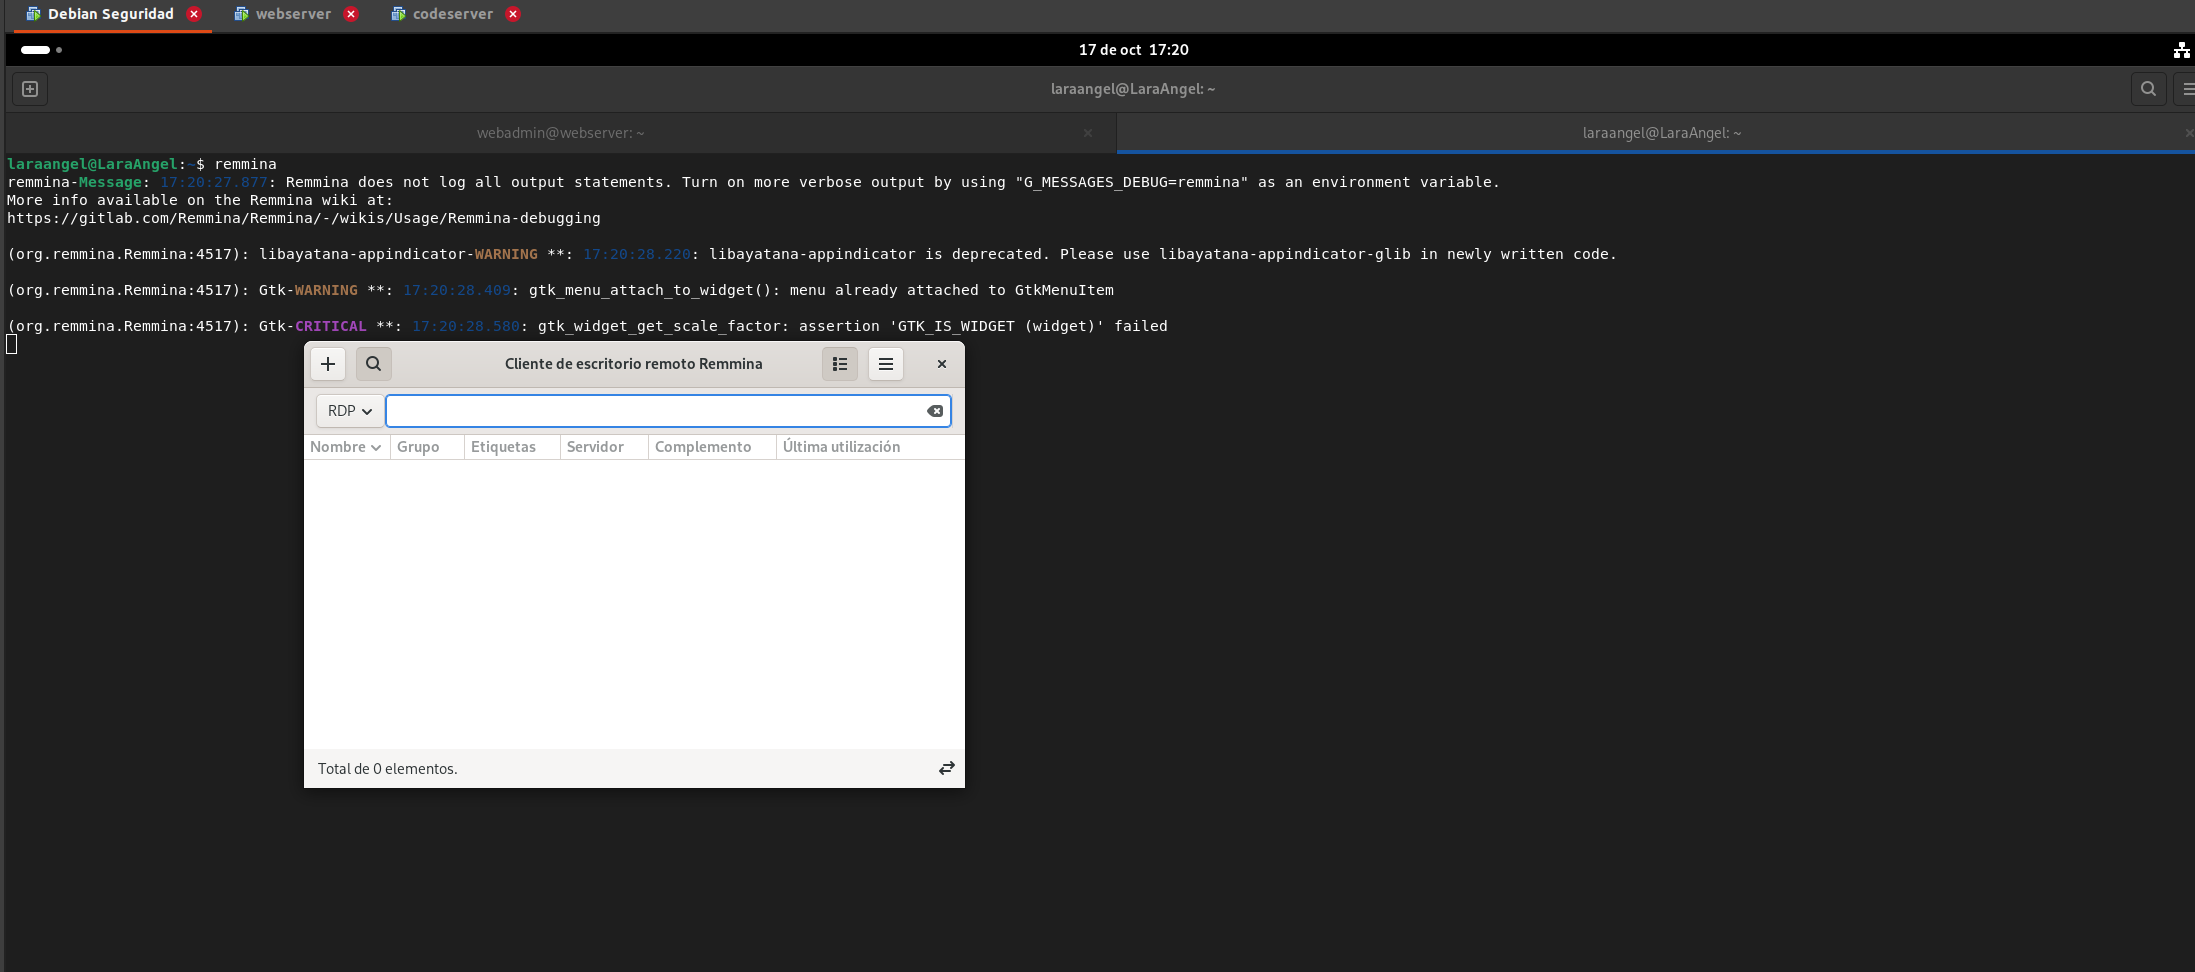
\includegraphics[width=0.8\textwidth,trim=265bp 170bp 570bp 340bp,clip]{img/image8.png}
    \caption{Ejecucion de la herramienta Remmina.}
\end{figure}

Ahora bien, la conexion se configura hacia \texttt{127.0.0.1},
utilizando el protocolo RDP y el puerto local 3389. Esto por que
Remmina se conecta al puerto del tunel en EvilBox y SSH se
encarga de llevar la conexion hasta codeserver.

\Needspace{8\baselineskip}
\subsection{Configuracion del perfil y conexion con codeserver}

En el primer intento, Remmina no logro establecer la conexion y
devolvio un error relacionado con TLS. Por lo que fue necesario
revisar la configuracion del perfil antes de continuar.

\begin{figure}[H]
    \centering
    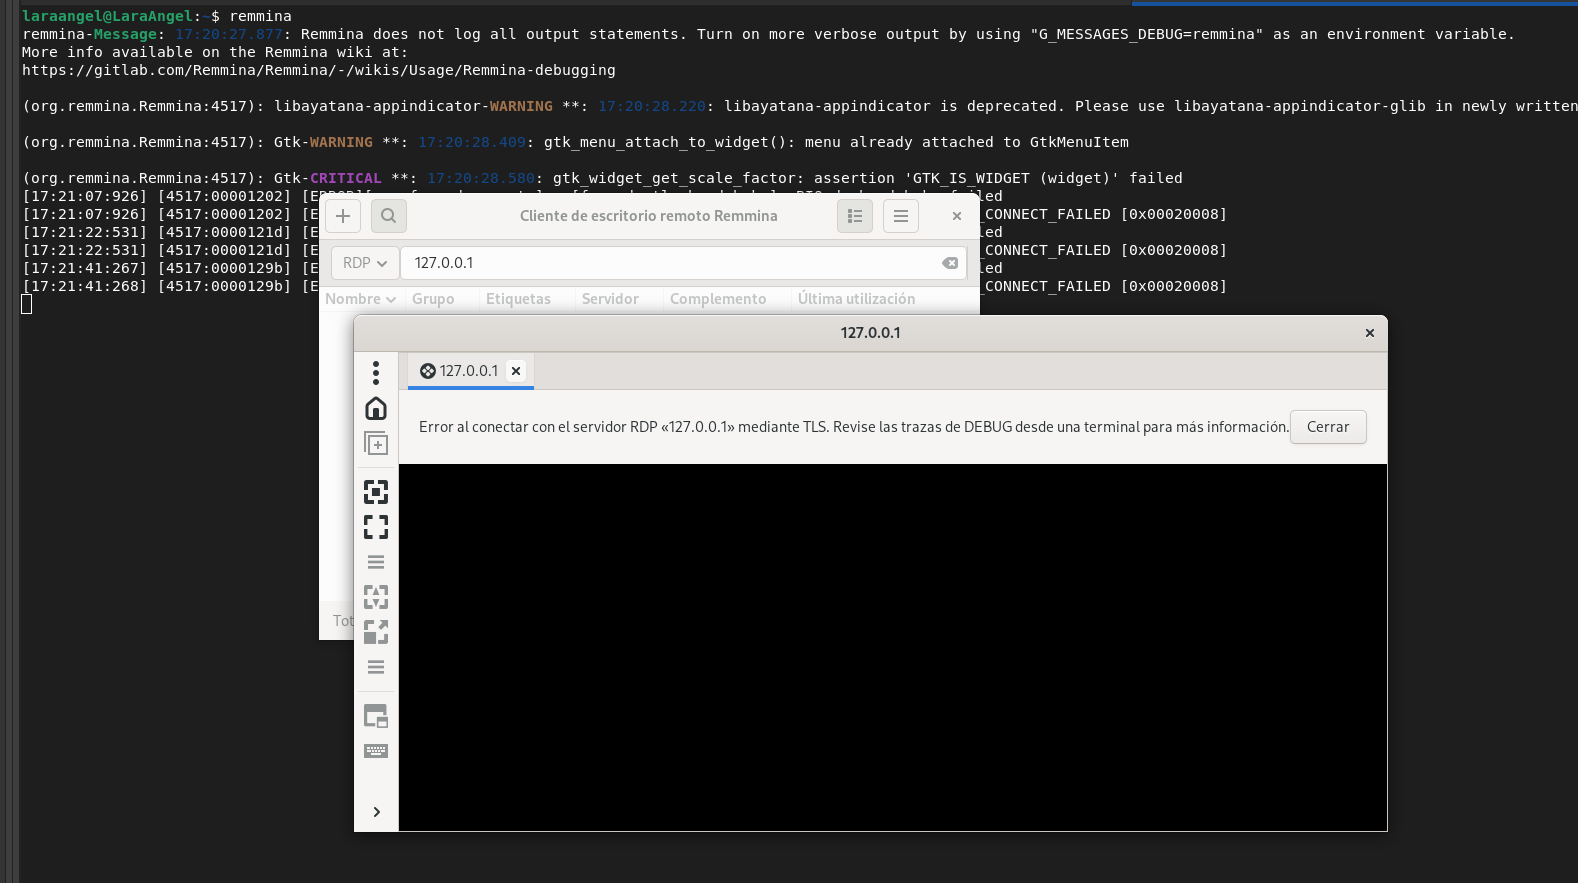
\includegraphics[width=\textwidth,trim=350bp 395bp 185bp 310bp,clip]{img/image9.png}
    \caption{Error de conexion RDP mediante TLS en el primer intento.}
\end{figure}

Para esto, se creo un perfil llamado Codeserver y se pusieron los
datos de la cuenta que se encontro en el archivo passwords.txt de
la practica 6. Los valores del perfil son los siguientes:

\begin{itemize}
    \item \textbf{Nombre:} Codeserver.
    \item \textbf{Protocolo:} RDP, protocolo de escritorio remoto.
    \item \textbf{Servidor:} 127.0.0.1, por el puerto local 3389.
    \item \textbf{Usuario:} developer2024.
    \item \textbf{Contraseña:} R0b0tRulz!.
    \item \textbf{Dominio:} se dejo vacio.
\end{itemize}

\begin{figure}[H]
    \centering
    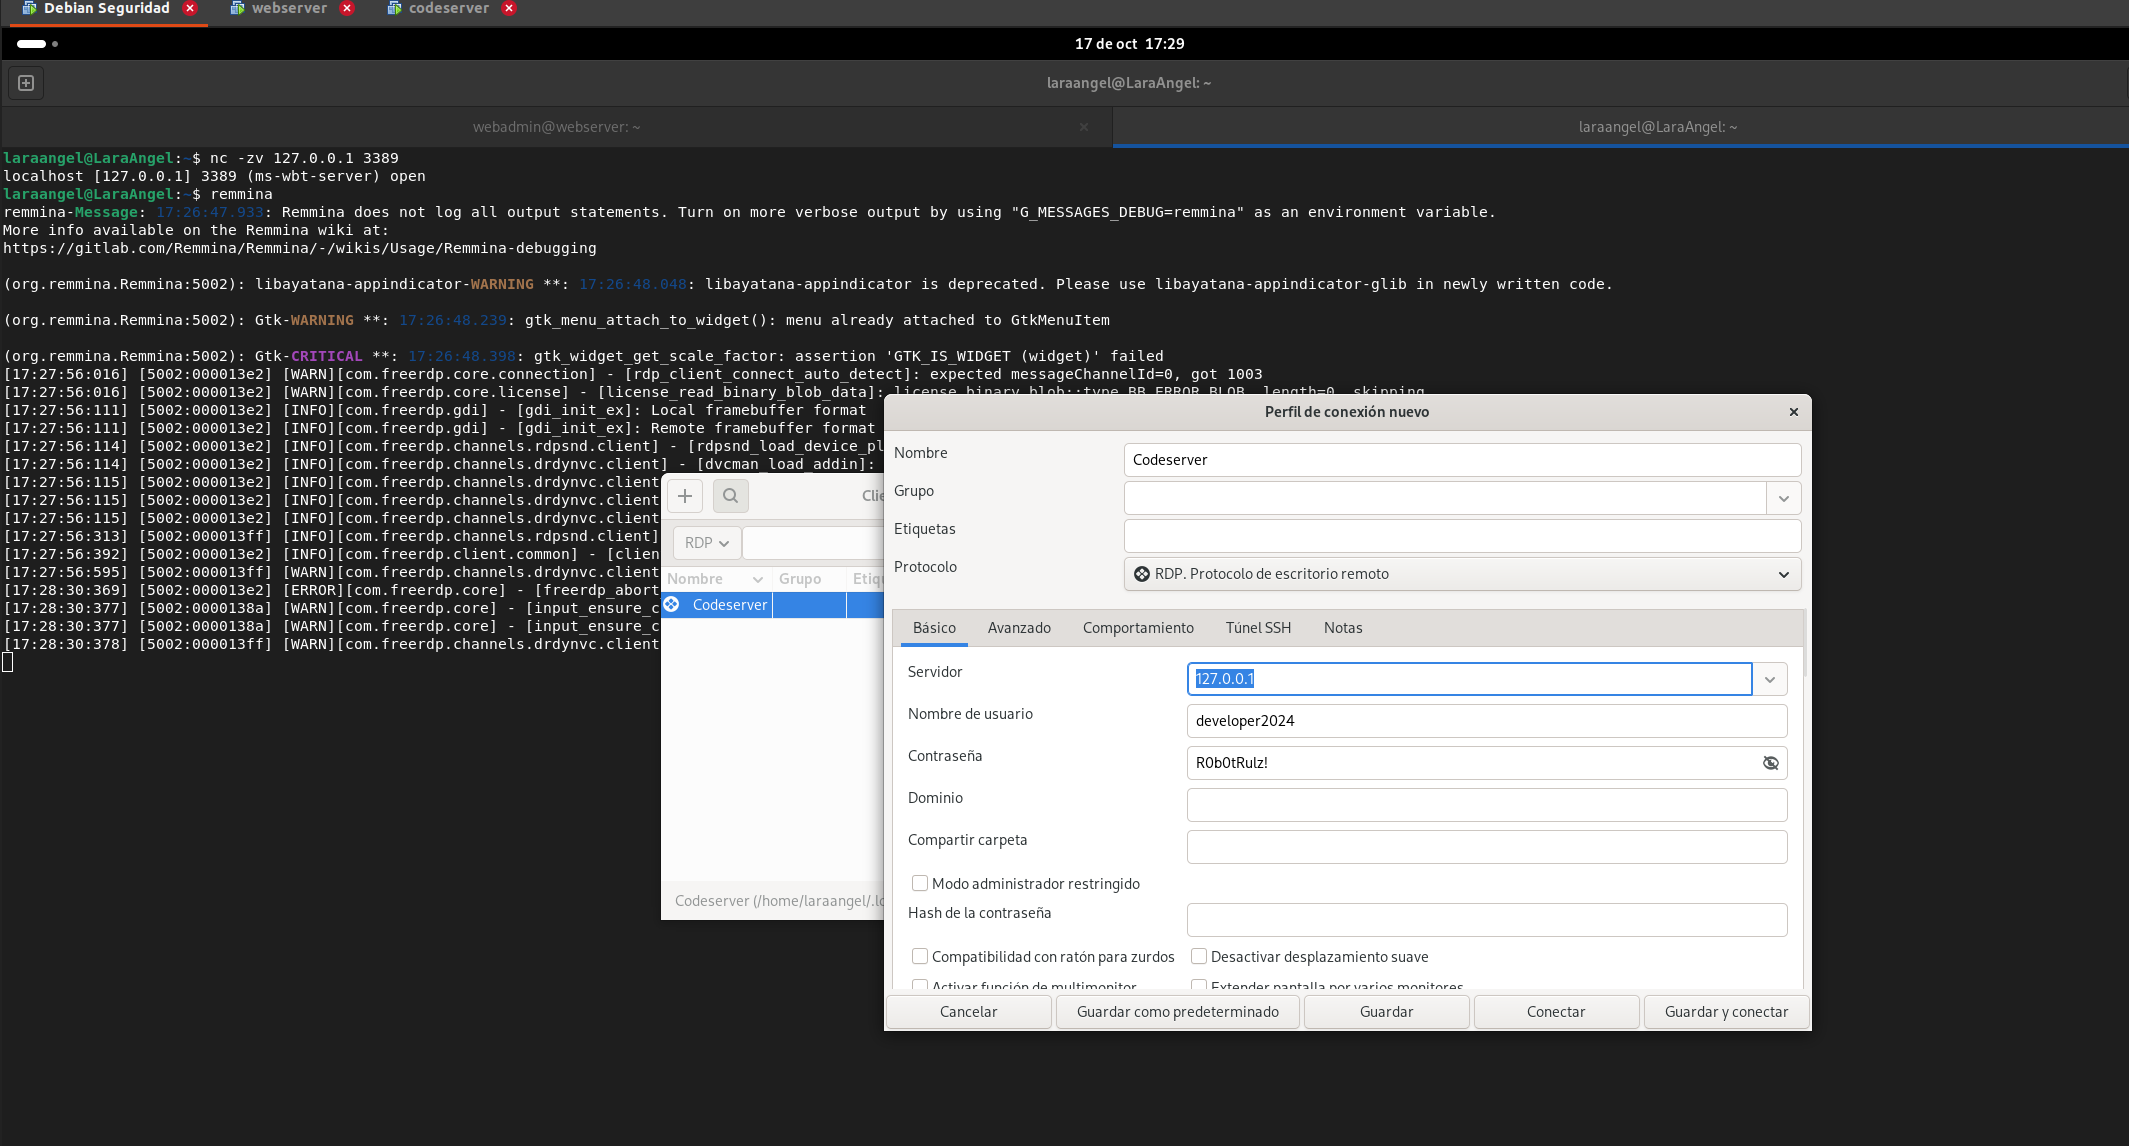
\includegraphics[width=\textwidth,trim=875bp 105bp 300bp 395bp,clip]{img/image10.png}
    \caption{Datos del perfil de conexion RDP para codeserver.}
\end{figure}

Donde en este caso, el usuario y la contraseña de codeserver son
distintos a los de webserver. La cuenta webadmin se utiliza para
la conexion SSH, mientras que developer2024 se utiliza para
ingresar al escritorio remoto del equipo Windows.

Despues de esto, en la pestaña Avanzado se selecciono
\textbf{Protocolo de seguridad RDP} en la negociacion del
protocolo de seguridad. Ademas de que, la calidad se dejo en
\textbf{Pobre (mas rapido)} y el nivel de seguridad de TLS quedo
en Predeterminados.

\begin{figure}[H]
    \centering
    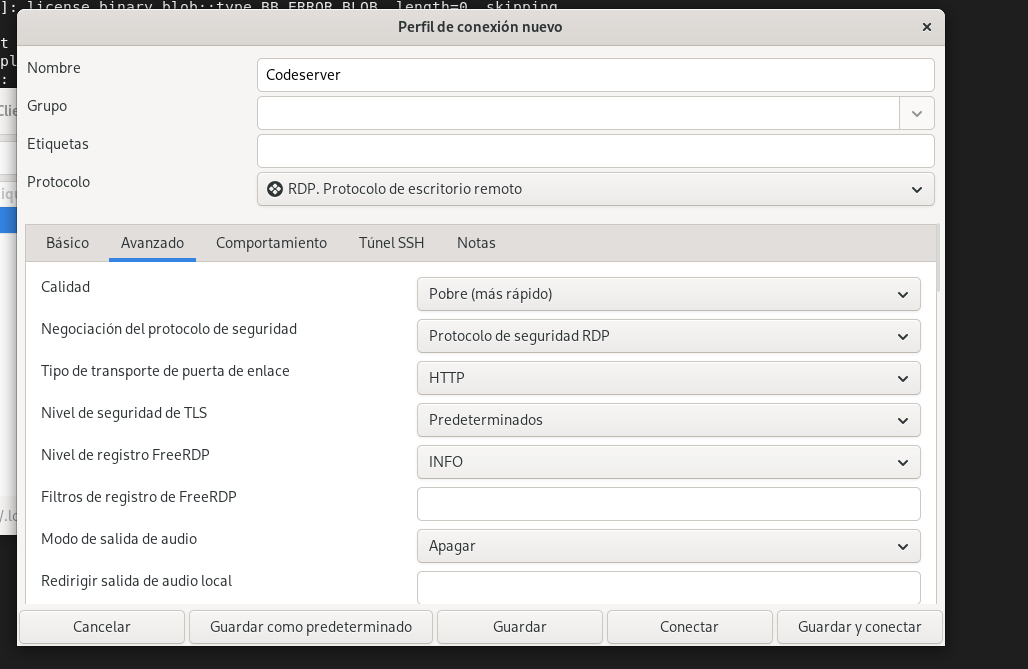
\includegraphics[width=0.9\textwidth,trim=20bp 225bp 80bp 220bp,clip]{img/image11.png}
    \caption{Configuracion avanzada del protocolo de seguridad RDP.}
\end{figure}

De igual forma, dentro de las opciones avanzadas se marco
\textbf{Ignorar certificado}. Estos fueron los ajustes utilizados
en el perfil de esta conexion para continuar con el acceso al
equipo del laboratorio.

\begin{figure}[H]
    \centering
    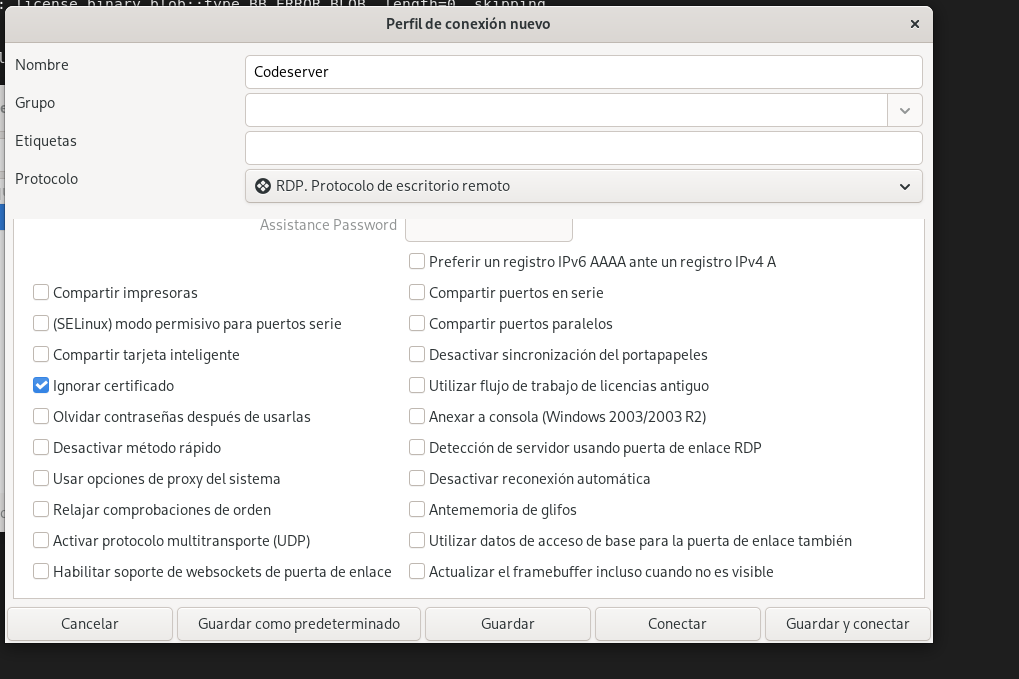
\includegraphics[width=0.65\textwidth,trim=20bp 270bp 639bp 370bp,clip]{img/image12.png}
    \caption{Opcion Ignorar certificado dentro del perfil de Remmina.}
\end{figure}

Una vez guardados los datos, se volvio a realizar la conexion con
el perfil Codeserver y se logro ingresar al escritorio de
Windows. Con esto ya tenemos acceso al otro equipo por medio de
RDP, utilizando el tunel que pasa por webserver.

\begin{figure}[H]
    \centering
    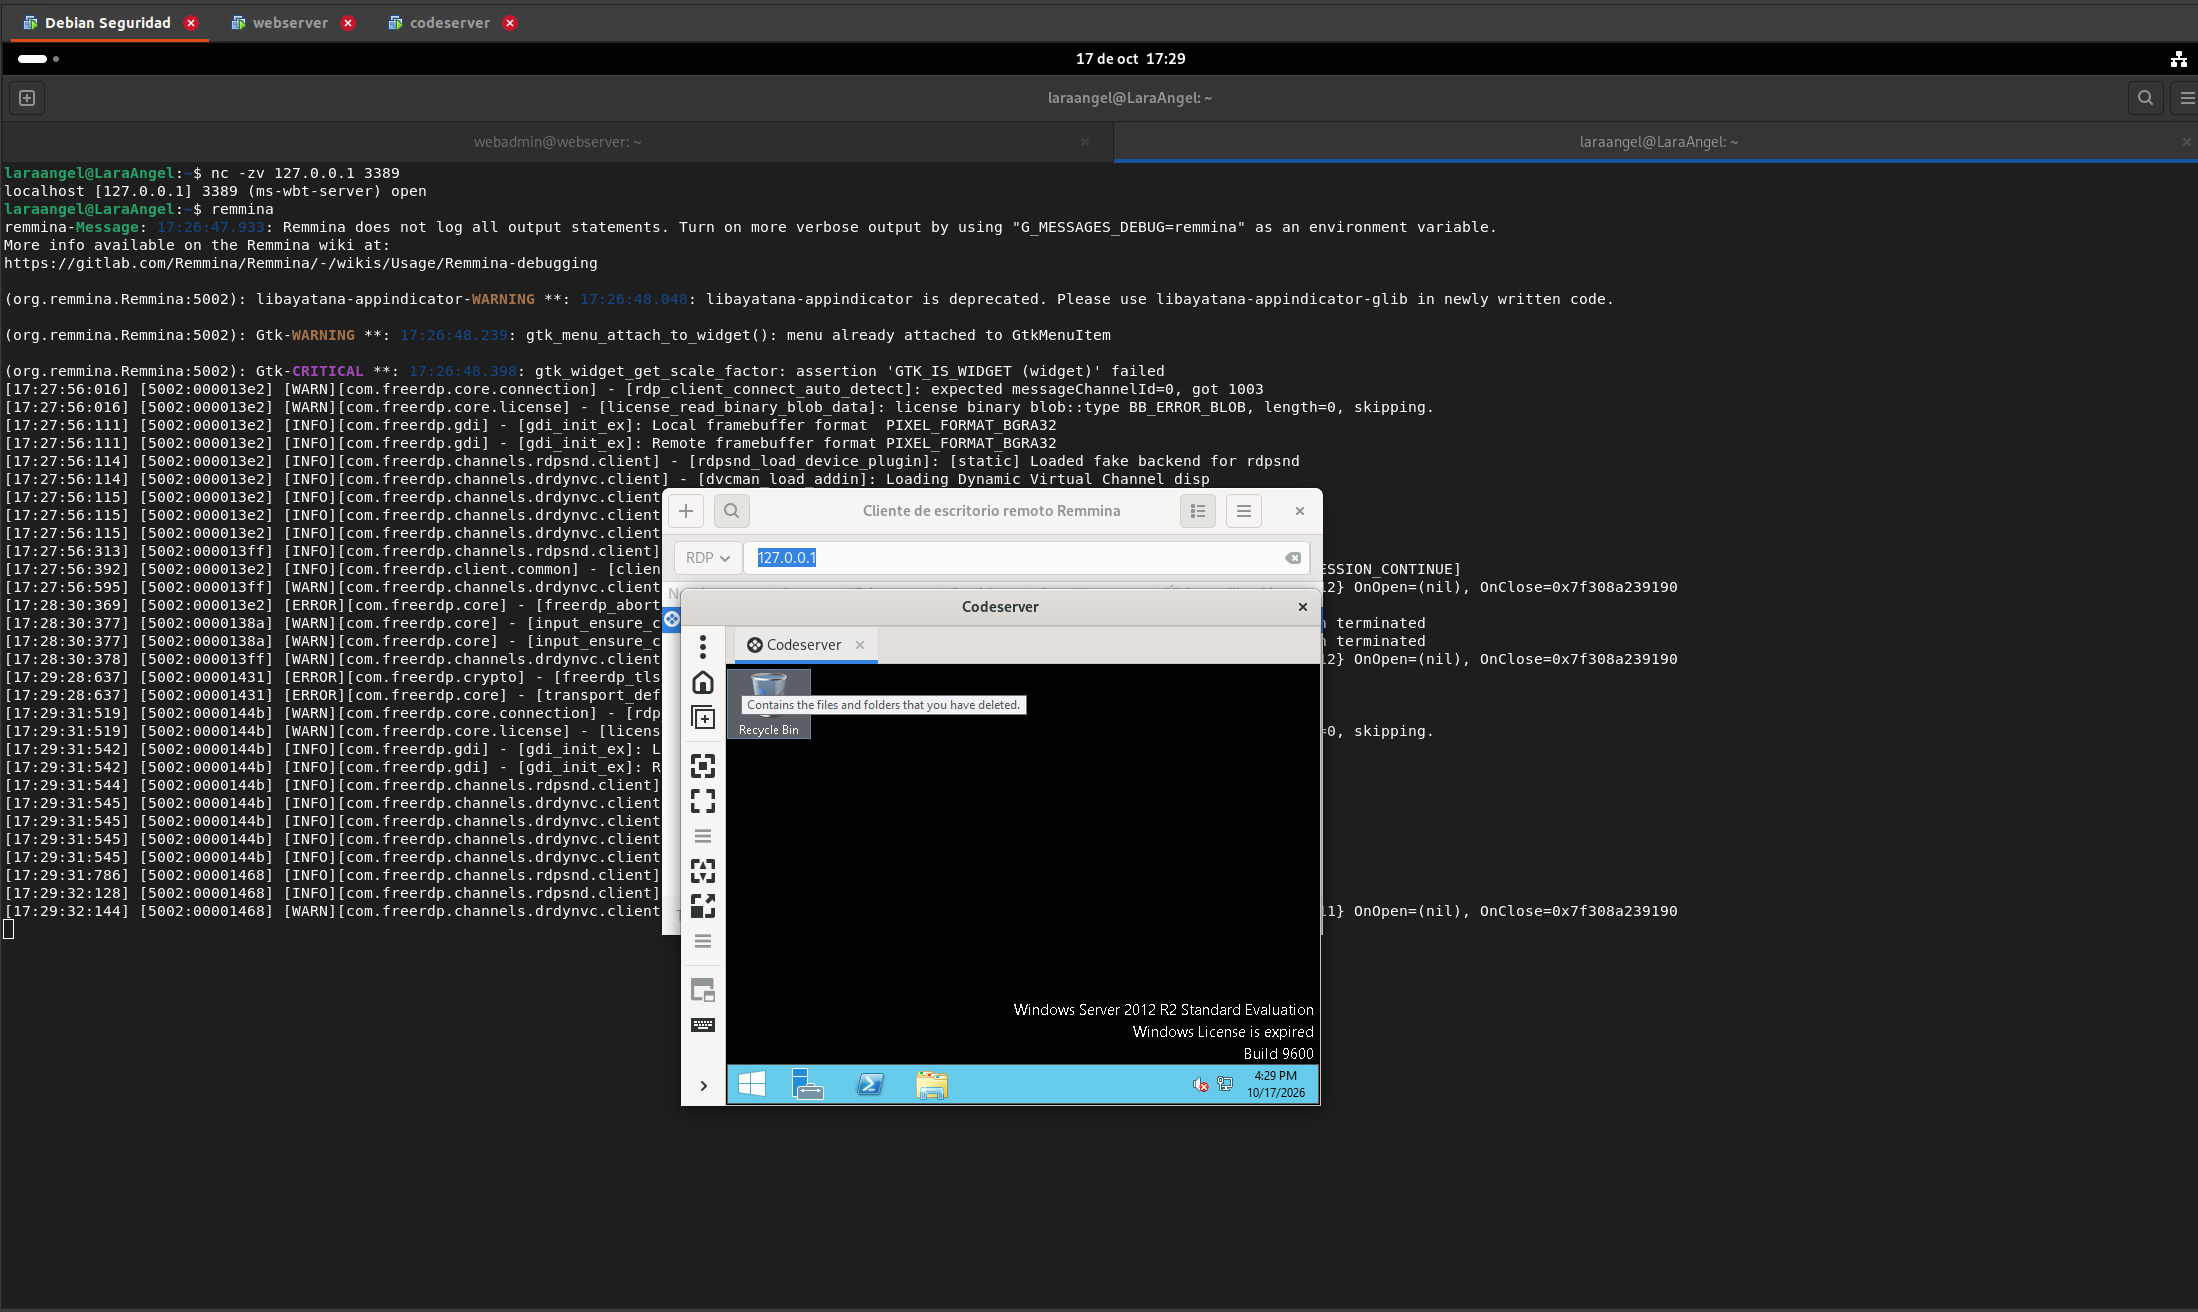
\includegraphics[width=0.75\textwidth,trim=660bp 180bp 840bp 485bp,clip]{img/image13.png}
    \caption{Sesion de escritorio remoto establecida con codeserver.}
\end{figure}

Por lo que, el movimiento lateral se realiza al utilizar las
credenciales encontradas y la comunicacion que tiene webserver
con la red interna para entrar a codeserver. A partir de esta
sesion se revisa la informacion del sistema y los archivos que se
piden en las actividades.

\newpage
\section{Actividades}

\Needspace{8\baselineskip}
\subsection{Actividad 1: Comando SSH para utilizar el puerto local 3389}

\textbf{¿Cual es el comando de SSH necesario para establecer una
conexion desde evilbox hacia codeserver, asumiendo que el puerto
local a utilizar es el 3389?}

Para esto, utilizamos el comando con el que se creo el tunel
durante el desarrollo:

\begin{lstlisting}[style=consolaSeguridad]
ssh -p 13337 -L 3389:10.0.0.201:3389 webadmin@192.168.177.129
\end{lstlisting}

Donde el puerto local es el primer 3389 de la opcion -L, la
direccion de codeserver es \texttt{10.0.0.201} y el puerto de
destino tambien es el 3389. La conexion SSH se realiza con
webadmin hacia webserver, por el puerto 13337.

Despues de crear el tunel, Remmina se conecta a
\texttt{127.0.0.1:3389} en EvilBox. La contraseña que se solicita
al ejecutar SSH es toronto, mientras que las credenciales de
Windows se escriben despues en el perfil RDP.

\Needspace{8\baselineskip}
\subsection{Actividad 2: Credenciales validas de codeserver}

\textbf{¿Cuales son las credenciales validas para ingresar al
equipo codeserver? Utilice el formato usuario:contraseña.}

Las credenciales que se utilizaron en Remmina son las que se
encontraron dentro del respaldo de ProjectX en la practica 6. En
el formato solicitado, la respuesta es la siguiente:

\begin{lstlisting}[style=output]
developer2024:R0b0tRulz!
\end{lstlisting}

Donde el usuario es developer2024 y la contraseña es R0b0tRulz!,
respetando los ceros, las mayusculas y el signo de admiracion al
final. Con esta cuenta se logro ingresar al escritorio remoto de
codeserver.

\begin{figure}[H]
    \centering
    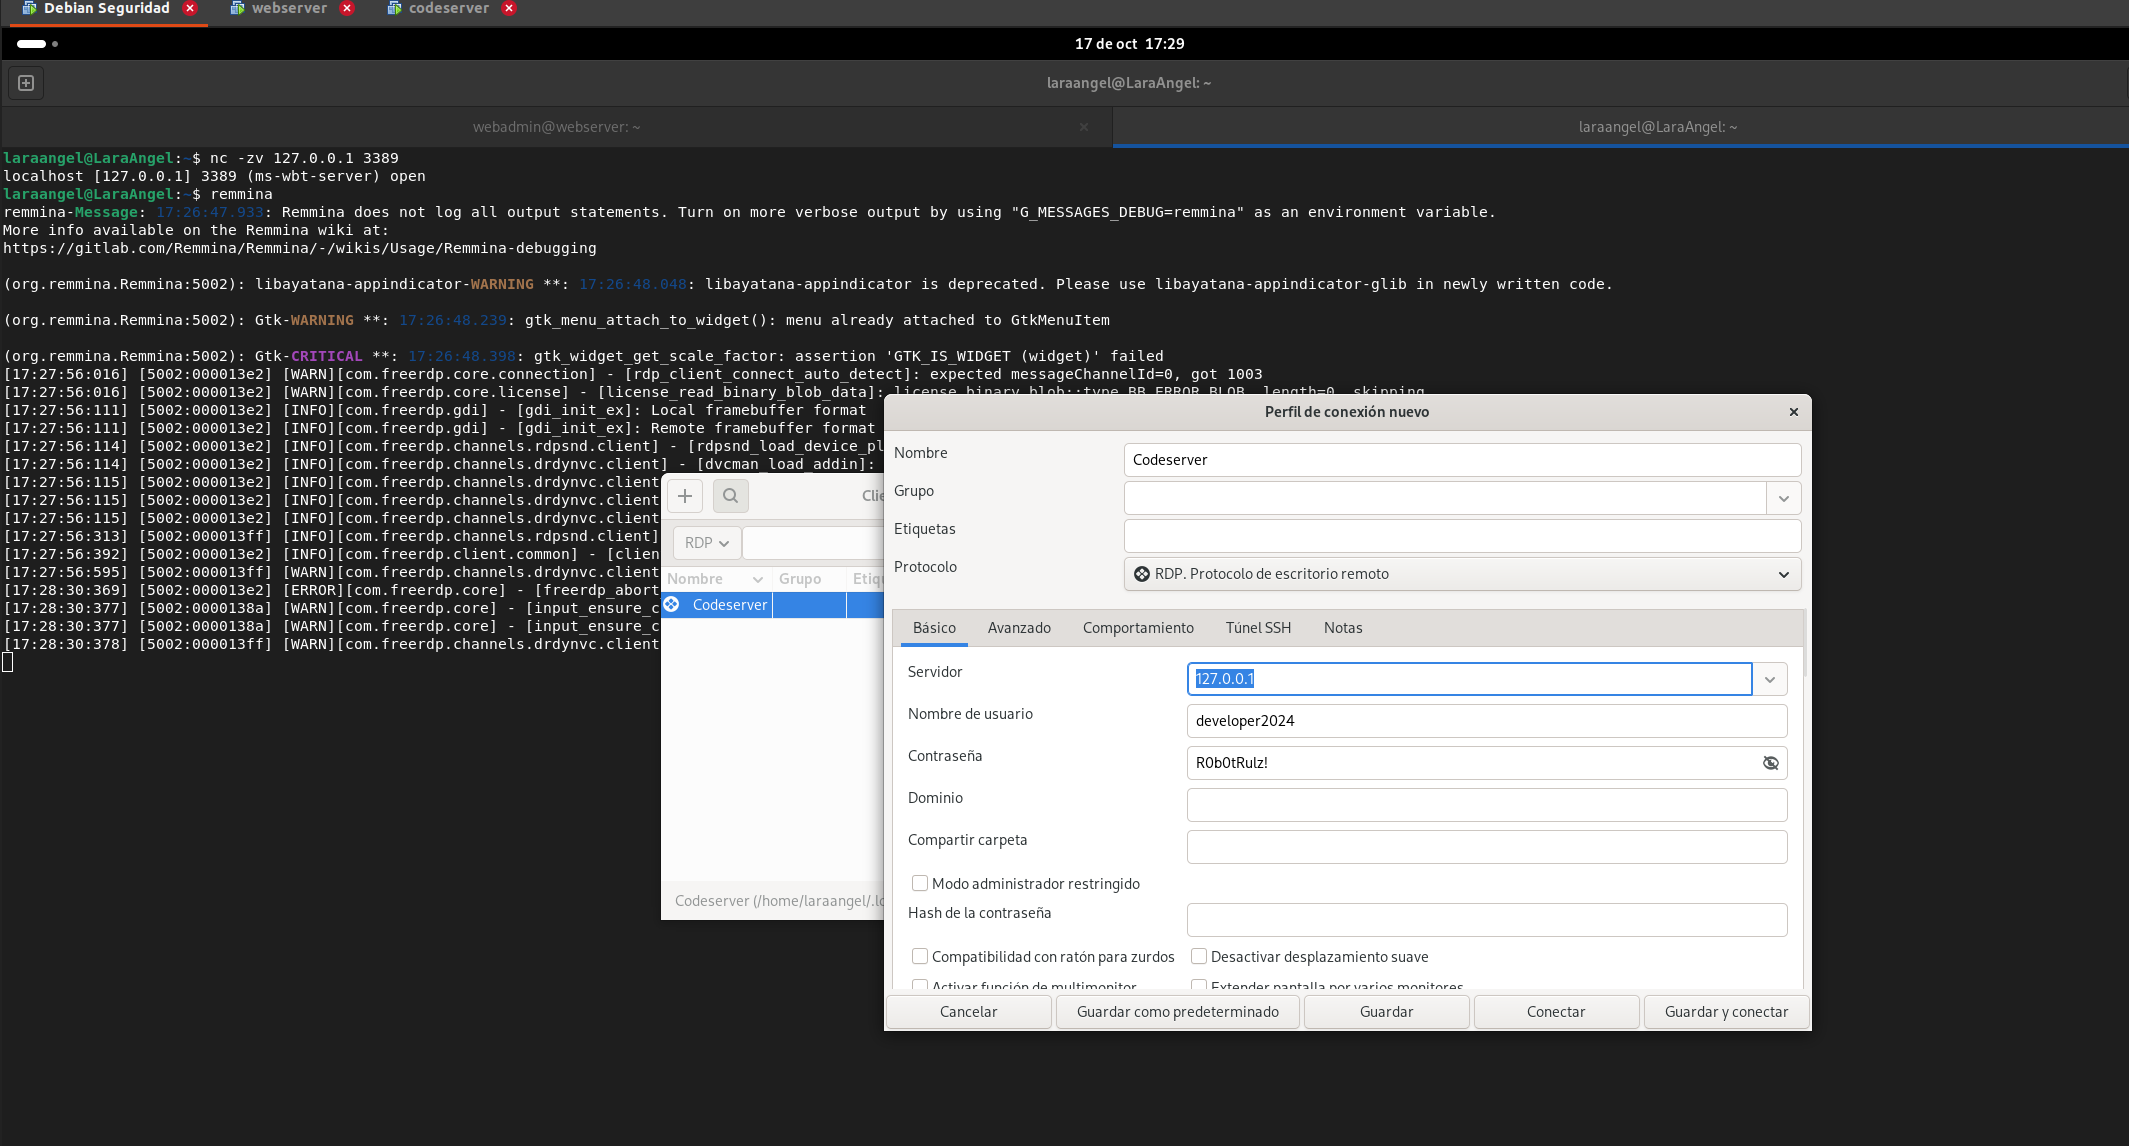
\includegraphics[width=\textwidth,trim=900bp 356bp 310bp 700bp,clip]{img/image10.png}
    \caption{Usuario y contraseña utilizados para la sesion RDP.}
\end{figure}

\Needspace{12\baselineskip}
\subsection{Actividad 3: Cuenta que permite la conexion remota}

\textbf{¿Cual es el nombre de la cuenta de usuario que permite la
conexion remota?}

La cuenta que permite la conexion remota al equipo codeserver es
la siguiente:

\begin{lstlisting}[style=output]
developer2024
\end{lstlisting}

Esta es la cuenta que se configuro en el perfil de Remmina y con
la que se establecio la sesion de Windows. Por otro lado,
webadmin corresponde al acceso SSH a webserver, que se utiliza
para mantener el tunel.

\Needspace{8\baselineskip}
\subsection{Actividad 4: Sistema operativo de codeserver}

\textbf{¿Cual es el sistema operativo instalado en el equipo
codeserver?}

Para revisar la informacion del sistema, se abrio la consola de
comandos dentro de la sesion remota y se utilizo systeminfo. Para
mostrar solamente el nombre y la version del sistema, se puede
filtrar de la siguiente forma:

\begin{lstlisting}[style=consolaWindows]
systeminfo | findstr /B /C:"OS Name" /C:"OS Version"
\end{lstlisting}

Donde \texttt{systeminfo} muestra la informacion del equipo y la
tuberia pasa el resultado a \texttt{findstr}. La opcion
\texttt{/B} busca las coincidencias al inicio de la linea y cada
\texttt{/C} permite buscar una cadena completa.

\begin{figure}[H]
    \centering
    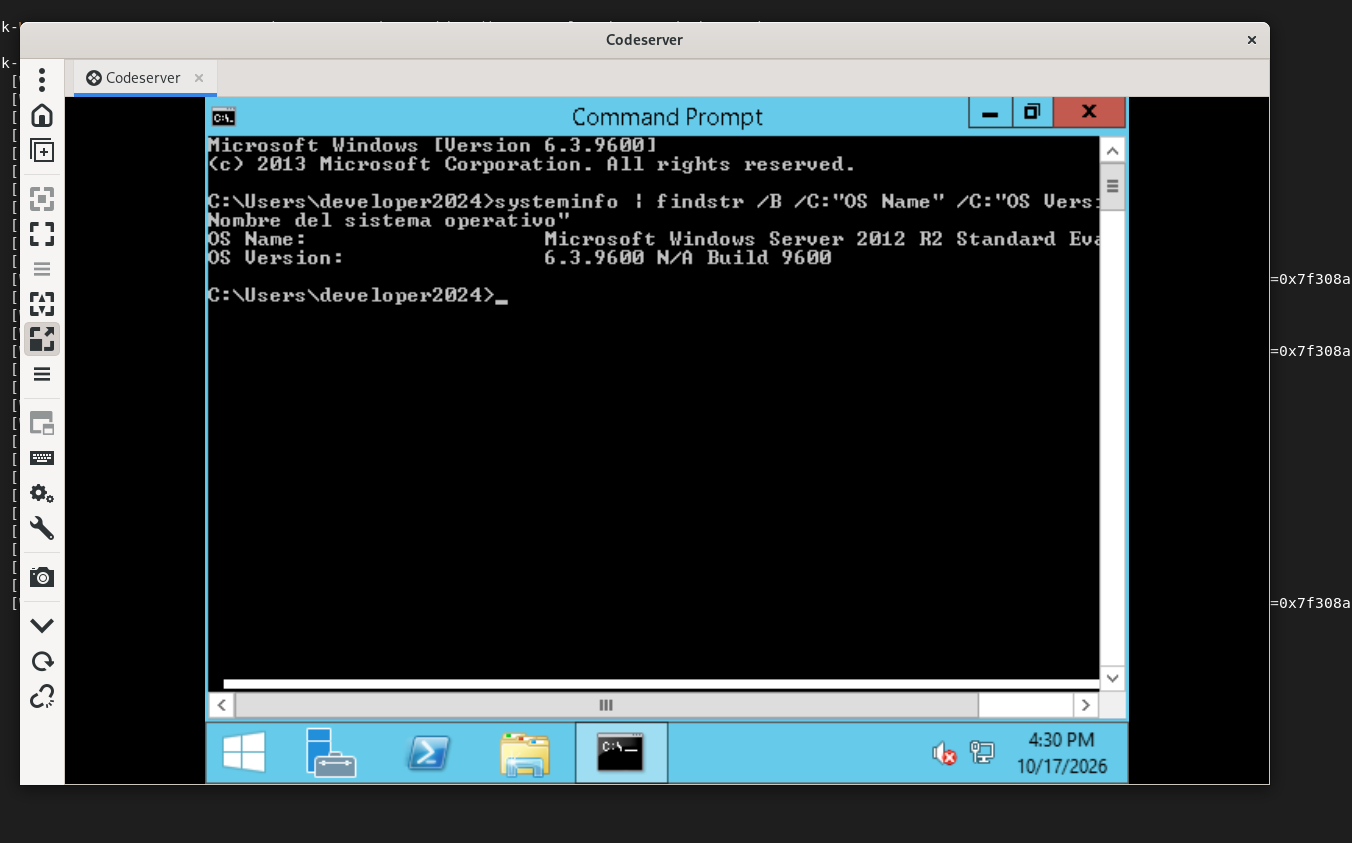
\includegraphics[width=\textwidth,trim=200bp 500bp 210bp 130bp,clip]{img/image14.png}
    \caption{Consulta del nombre y version del sistema operativo.}
\end{figure}

El sistema operativo instalado es \textbf{Microsoft Windows
Server 2012 R2 Standard Evaluation}. La version que devuelve el
equipo es la siguiente:

\begin{lstlisting}[style=output]
OS Version: 6.3.9600 N/A Build 9600
\end{lstlisting}

Con esto podemos ver que se trata de la compilacion 9600 de
Windows Server 2012 R2. El nombre de la edicion tambien se
identifica dentro del escritorio remoto.

\Needspace{8\baselineskip}
\subsection{Actividad 5: Contenido de la etiqueta title}

\textbf{¿Cual es el contenido de la etiqueta HTML title de la
pagina web alojada en el equipo codeserver?}

Para esto, primero se localizo el archivo index.html y despues se
reviso el que se encuentra en el directorio del sitio web. Para
obtener solamente la linea del titulo, se puede utilizar el
siguiente comando:

\begin{lstlisting}[style=consolaWindows]
type "C:\inetpub\wwwroot\index.html" | findstr /i "title"
\end{lstlisting}

Lo que hace \texttt{type} es mostrar el contenido del archivo,
mientras que \texttt{findstr /i} busca la cadena title sin
distinguir entre mayusculas y minusculas. El resultado obtenido
es el siguiente:

\begin{lstlisting}[style=output]
<title>Chatbot</title>
\end{lstlisting}

\begin{figure}[H]
    \centering
    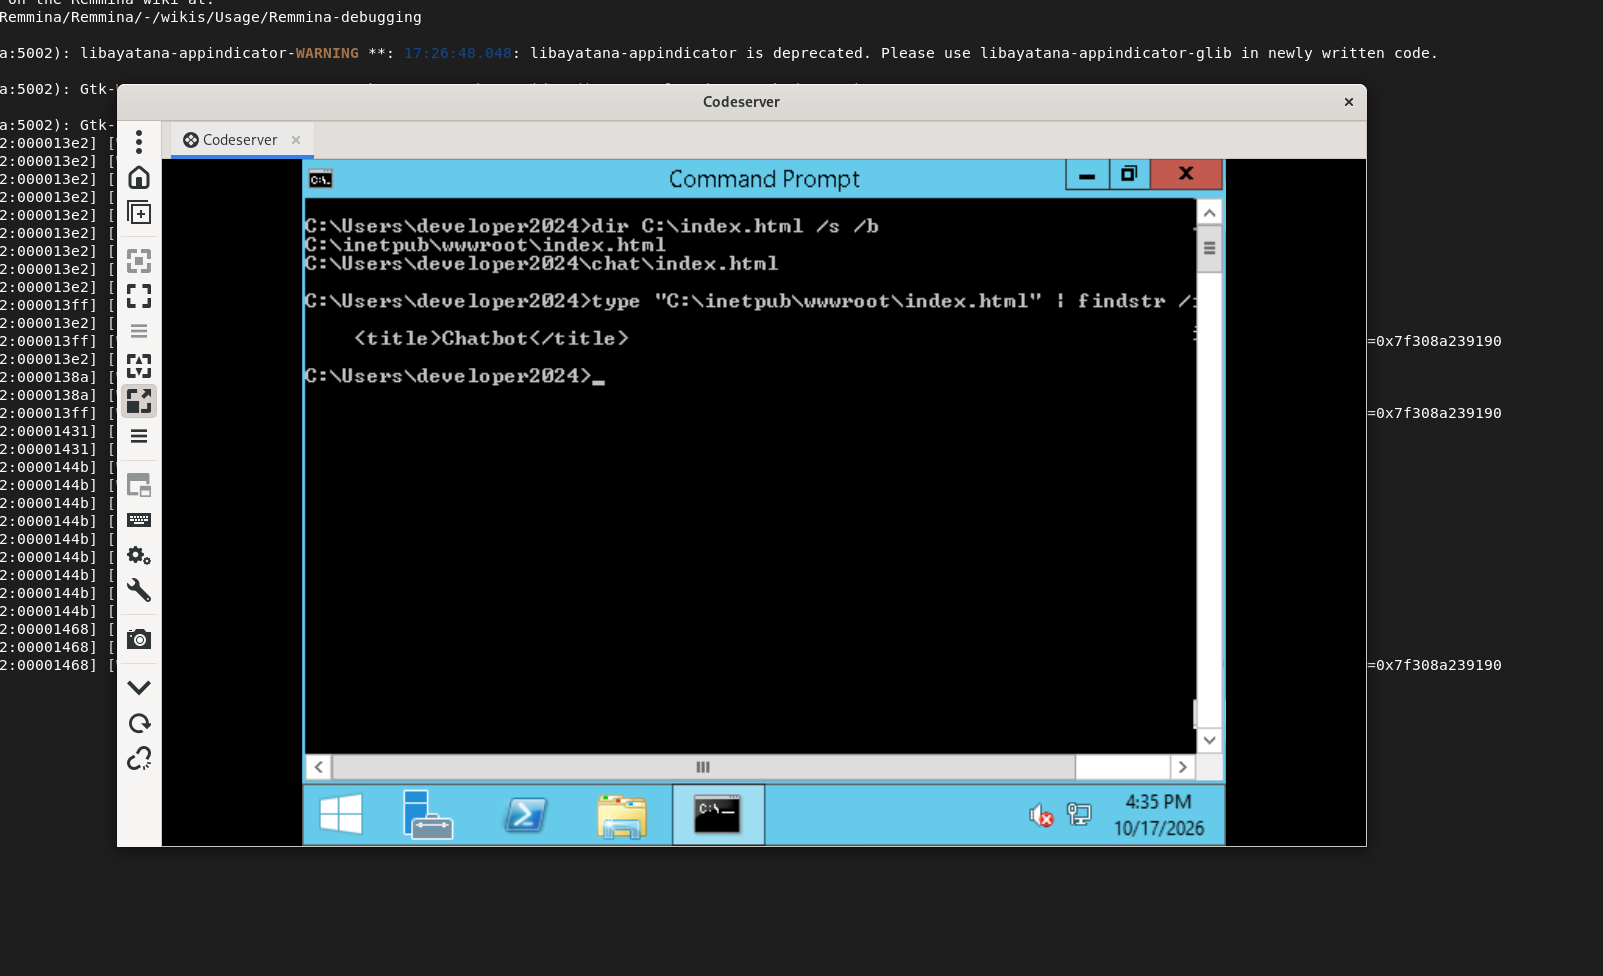
\includegraphics[width=\textwidth,trim=315bp 550bp 350bp 200bp,clip]{img/image15.png}
    \caption{Revision de la etiqueta title del archivo index.html.}
\end{figure}

Por lo que, el contenido de la etiqueta title es
\textbf{Chatbot}, con la C mayuscula. Las etiquetas de apertura y
cierre son parte del HTML, mientras que Chatbot es el texto que
contienen.

\Needspace{8\baselineskip}
\subsection{Actividad 6: Ruta absoluta de index.html}

\textbf{¿Cual es la ruta absoluta del archivo index.html ubicado
en el equipo codeserver?}

Para encontrar el archivo se utilizo el comando dir con una
busqueda dentro de la unidad C. El comando es el siguiente:

\begin{lstlisting}[style=consolaWindows]
dir C:\index.html /s /b
\end{lstlisting}

Donde \texttt{/s} permite revisar tambien los subdirectorios y
\texttt{/b} muestra las rutas sin agregar el encabezado ni los
datos de tamaño y fecha. El resultado nos arroja dos archivos:

\begin{lstlisting}[style=output]
C:\inetpub\wwwroot\index.html
C:\Users\developer2024\chat\index.html
\end{lstlisting}

\begin{figure}[H]
    \centering
    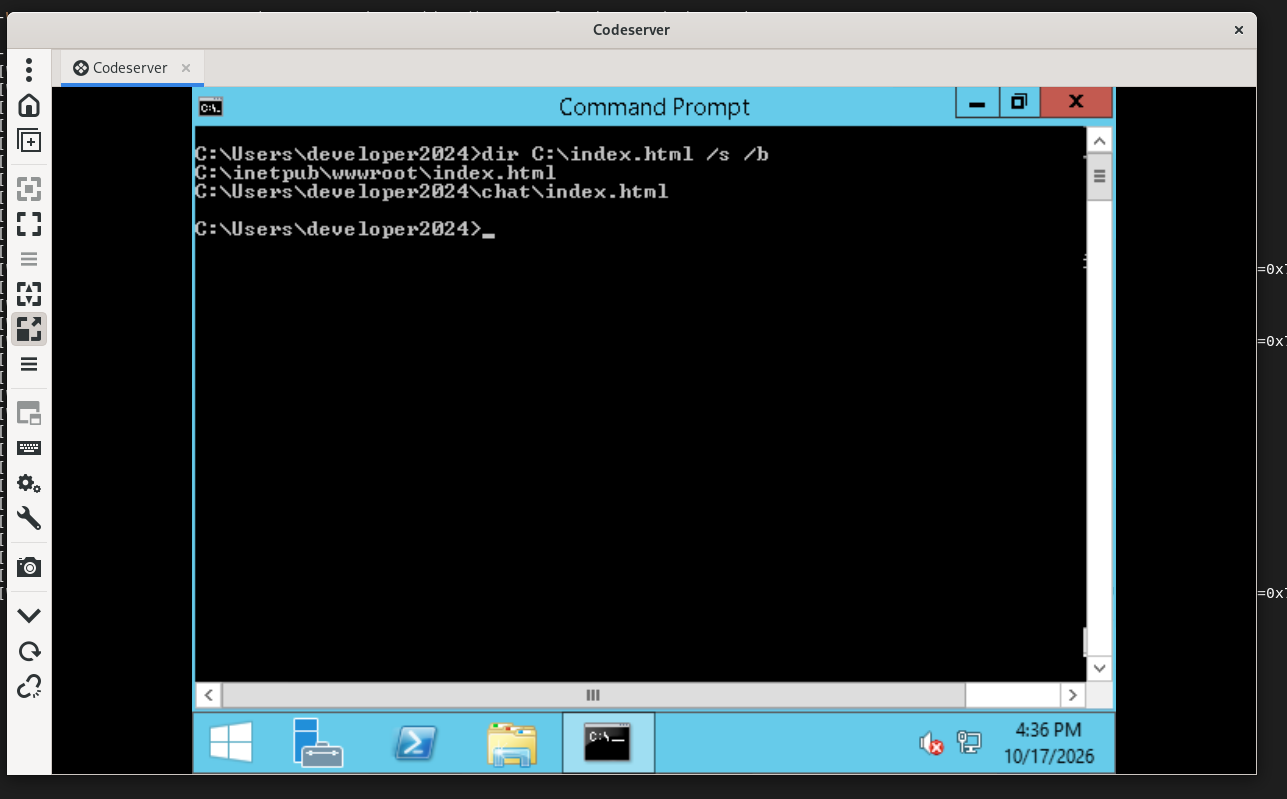
\includegraphics[width=\textwidth,trim=180bp 530bp 210bp 130bp,clip]{img/image16.png}
    \caption{Busqueda de index.html dentro de la unidad C.}
\end{figure}

Donde en este caso, para la pagina web se toma la primera ruta,
que corresponde al archivo index.html dentro del directorio
wwwroot. La otra ruta corresponde a una copia dentro del
directorio chat del usuario developer2024.

\Needspace{8\baselineskip}
\subsection{Actividad 7: Archivo con el codigo fuente del chatbot}

\textbf{¿Cual es el nombre del archivo que tiene el codigo fuente
del chatbot?}

Para responder esta actividad se revisaron los archivos del
directorio del sitio web y del directorio chat del usuario. Los
comandos son los siguientes:

\begin{lstlisting}[style=consolaWindows]
dir C:\inetpub\wwwroot\ /b
dir C:\Users\developer2024\chat\ /b
\end{lstlisting}

Donde en este caso, el directorio wwwroot contiene los siguientes
archivos:

\begin{lstlisting}[style=output]
bot.py
configuracion.ini
index.html
script.js
styles.css
\end{lstlisting}

\begin{figure}[H]
    \centering
    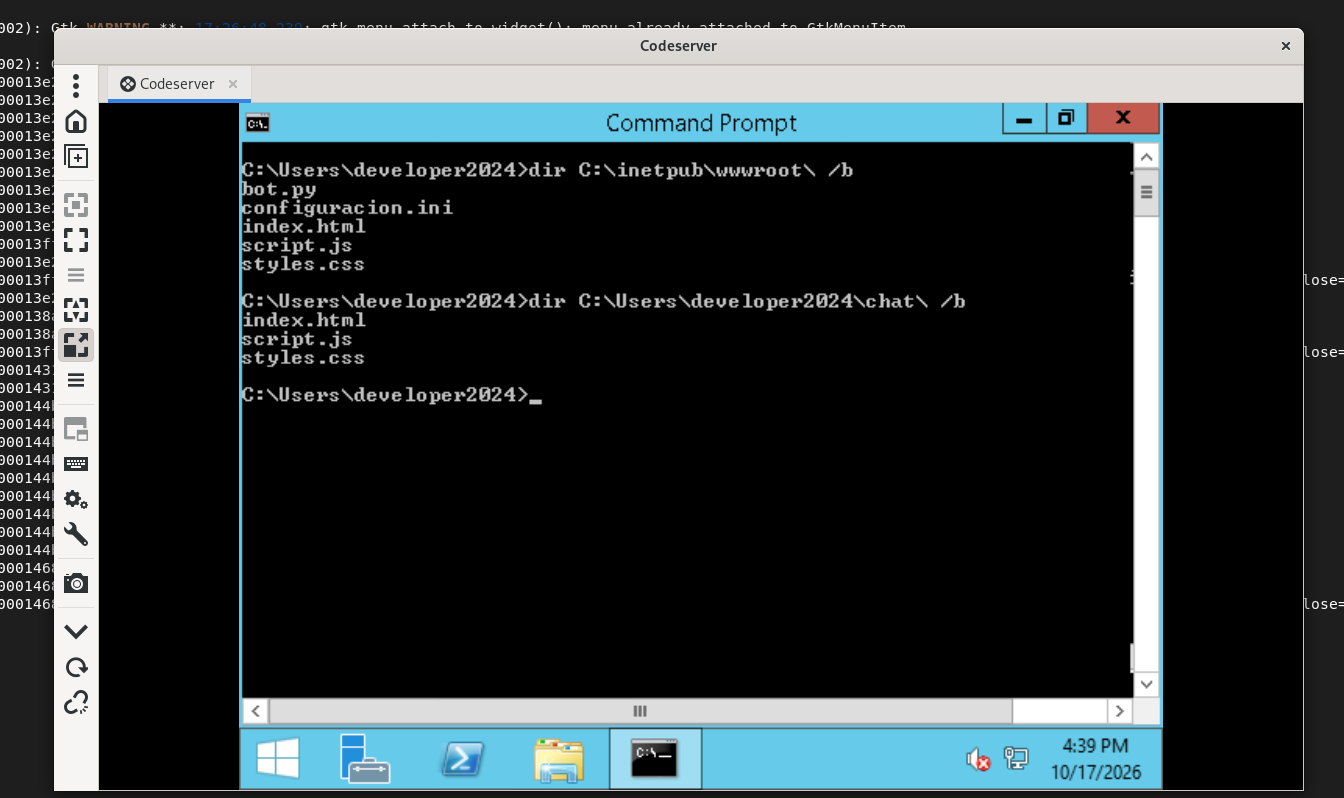
\includegraphics[width=\textwidth,trim=230bp 421bp 190bp 140bp,clip]{img/image17.png}
    \caption{Archivos del sitio web y del directorio chat.}
\end{figure}

Por otro lado, dentro de chat aparecen index.html, script.js y
styles.css. El archivo identificado como codigo fuente del
chatbot es \textbf{bot.py}, ubicado en el directorio wwwroot
del servidor web. La extension
py corresponde a un archivo de Python.

\Needspace{26\baselineskip}
\subsection{Actividad 8: Hash SHA256 del codigo fuente}

\textbf{¿Cual es el hash SHA256 del archivo que tiene el codigo
fuente del chatbot?}

Para obtener el hash del archivo bot.py se utilizo certutil
dentro de la consola de Windows. El comando completo es el
siguiente:

\begin{lstlisting}[style=consolaWindows]
certutil -hashfile "C:\inetpub\wwwroot\bot.py" SHA256
\end{lstlisting}

Donde \texttt{-hashfile} indica que se va a calcular el hash de
un archivo, despues se pone la ruta completa de bot.py y al final
se especifica el algoritmo SHA256. La salida muestra el hash
separado en pares de caracteres, de la siguiente forma:

\begin{lstlisting}[style=hashCredencial]
b4 94 a0 d1 fc 37 d7 16 ab 00 69 4e da 6f 35 95
f6 4f e7 b9 75 91 a8 b5 f1 3e 9f 90 a7 22 36 49
\end{lstlisting}

\begin{figure}[H]
    \centering
    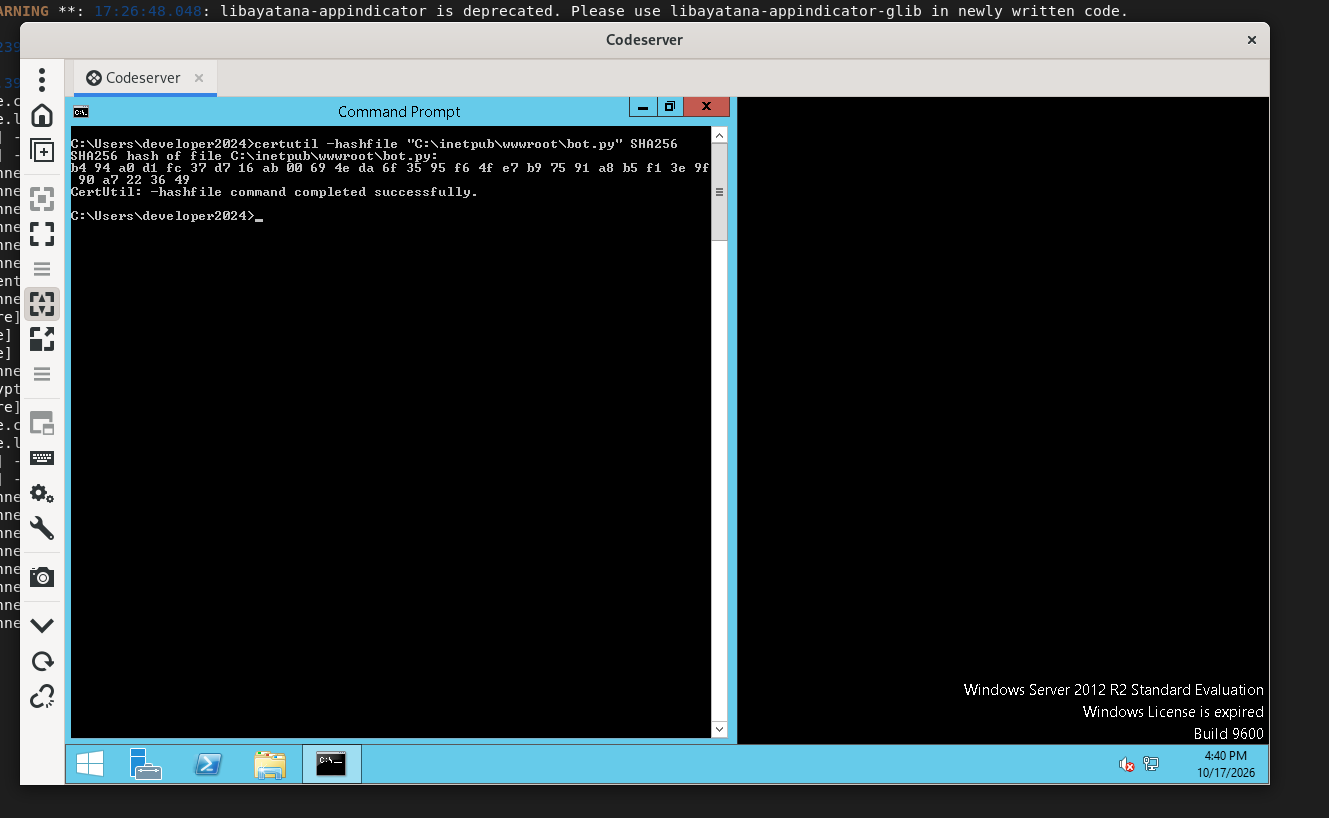
\includegraphics[width=\textwidth,trim=65bp 575bp 600bp 125bp,clip]{img/image18.png}
    \caption{Calculo del hash SHA256 del archivo bot.py.}
\end{figure}

Ahora bien, para escribir el resultado como una sola cadena, se
quitan los espacios entre los pares, conservando los mismos
valores. Por lo que el hash SHA256 es el siguiente:

\Needspace{4\baselineskip}

\begin{lstlisting}[style=hashCredencial]
b494a0d1fc37d716ab00694eda6f3595f64fe7b97591a8b5f13e9f90a7223649
\end{lstlisting}

Este valor corresponde al contenido del archivo bot.py que se
reviso en codeserver. Ademas de que, la salida de certutil indica
que el comando termino correctamente.

\newpage
\nocite{*}
\printbibliography[heading=bibintoc,title={Referencias}]
\end{document}
